\documentclass[conference]{IEEEtran}
\IEEEoverridecommandlockouts
% The preceding line is only needed to identify funding in the first footnote. If that is unneeded, please comment it out.
%Template version as of 6/27/2024

% \usepackage{xcolor}
\usepackage[table,usenames,dvipsnames]{xcolor}

\usepackage{amsmath,amssymb,amsfonts}
\usepackage{graphicx}

\usepackage{nameref}

% For abbreviations, we use "acro" package, and mfirstuc to help capitalize long
% versions normally
\usepackage{mfirstuc}
\MFUhyphentrue % tell mfirstuc to capitalize hyphenated words

% Acronyms
\usepackage{acro}
% For one-offs,
% \DeclareAcronym{acronym}{short=short-version,long=long-version}

\newcommand{\newacr}[2]{\DeclareAcronym{#1}{short=\uppercase{#1},long=#2}}
\newcommand{\newacrs}[3]{\DeclareAcronym{#1}{short=#2,long=#3}}

% Alphabetically sorted list of acronyms
\newacr{aop}{Aspect-Oriented Programming}
\newacr{api}{Application Programming Interface}
\newacr{ast}{Abstract Syntax Tree}
\newacr{cms}{Content Management System}
\newacr{cpu}{Central Processing Unit}
\newacr{csv}{Comma-Separated Values}
\newacr{dsl}{Domain-Specific Language}
\newacr{ffi}{Foreign Function Interface}
\newacr{gui}{Graphical User Interface}
\newacr{html}{HyperText Markup Language}
\newacr{href}{Hypertext REFerence}
\newacr{ide}{Integrated Development Environment}
\newacr{json}{JavaScript Object Notation}
\newacr{jvm}{Java Virtual Machine}
\newacr{mop}{MetaObject Protocol}
\newacr{nasa}{National Aeronautics and Space Administration}
\newacr{pdf}{Portable Document Format}
\newacr{sst}{Skeleton Syntax Tree}
\newacr{wysiwyg}{What You See Is What You Get}

% Case Studies 
%   (note: I'm grouping these together and forcing "newacrs" usage, even when
%    seemingly unneeded because, otherwise, they won't group together at the 
%    bottom of the complete "acronyms" list.)
\newacrs{glassbr}{GlassBR}{Glass Breaking}
\newacrs{projectile}{Projectile}{Projectile}
\newacrs{sglpend}{SglPend}{Single Pendulum}
\newacrs{dblpend}{DblPend}{Double Pendulum}
\newacrs{gamephysics}{GamePhysics}{Game Physics}
\newacrs{hghc}{HGHC}{Heat Transfer Coefficients between Fuel and Cladding in Fuel Rods}
\newacrs{pdcontroller}{PDController}{Proportional Derivative Controller}
\newacrs{swhs}{SWHS}{Solar Water Heating System}
\newacrs{nopcm}{SWHSNoPCM}{Solar Water Heating System Without PCM}
\newacrs{ssp}{SSP}{Slope Stability analysis Program}


%------------------------------------------------------------------------------
%- Extra commands for more functionality -- in particular, capitalizing the
%- long form of acronyms.
%------------------------------------------------------------------------------

% Defining \ACL - to capitalize all words in an acronym
% Credits to: https://tex.stackexchange.com/a/257896
\NewDocumentCommand\ACF{sm}{%
  \begingroup
  \acsetup{uppercase/cmd=\ecapitalisewords}%
  \IfBooleanTF{#1}{\Acf*{#2}}{\Acf{#2}}%
  \endgroup
}

\NewDocumentCommand\ACFP{sm}{%
  \begingroup
  \acsetup{uppercase/cmd=\ecapitalisewords}%
  \IfBooleanTF{#1}{\Acfp*{#2}}{\Acfp{#2}}%
  \endgroup
}

\NewDocumentCommand\ACL{sm}{%
  \begingroup
  \acsetup{uppercase/cmd=\ecapitalisewords}%
  \IfBooleanTF{#1}{\Acl*{#2}}{\Acl{#2}}%
  \endgroup
}

\NewDocumentCommand\ACLP{sm}{%
  \begingroup
  \acsetup{uppercase/cmd=\ecapitalisewords}%
  \IfBooleanTF{#1}{\Aclp*{#2}}{\Aclp{#2}}%
  \endgroup
}


% General Assets
%------------------------------------------------------------------------------
% Code
%------------------------------------------------------------------------------

\input{assets/code/names}
\input{assets/misc/posterHelpers}

% for assets/code/example.tex...
\newcommand{\exampleCode}{\input{assets/code/example}}
\newcommand{\refExampleCode}{\Cref{lst:exampleCode}}

% for assets/code/examplePseudocode.tex...
\newcommand{\examplePseudocode}{\input{assets/code/examplePseudocode}}
\newcommand{\refExamplePseudocode}{\Cref{lst:examplePseudocode}}

% for assets/code/mainInvalidInputTest.tex...
\newcommand{\mainInvalidInputTest}{\input{assets/code/mainInvalidInputTest}}
\newcommand{\refMainInvalidInputTest}{\Cref{lst:mainInvalidInputTest}}

% for assets/code/projManualViolationReq.tex...
\newcommand{\projManualViolationReq}{\input{assets/code/projManualViolationReq}}
\newcommand{\refProjManualViolationReq}{\Cref{lst:projManualViolationReq}}

% for assets/code/projViolationChoice.tex...
\newcommand{\projViolationChoice}{\input{assets/code/projViolationChoice}}
\newcommand{\refProjViolationChoice}{\Cref{lst:projViolationChoice}}

%------------------------------------------------------------------------------
% Graphs
%------------------------------------------------------------------------------

% Organization of files

\newcommand{\parChdGraphs}{
    % Only top or bottom to comply with IEEE guidelines
    \begin{figure}[bt!]
        \centering
        \begin{subfigure}[b]{\linewidth}
            \centering
            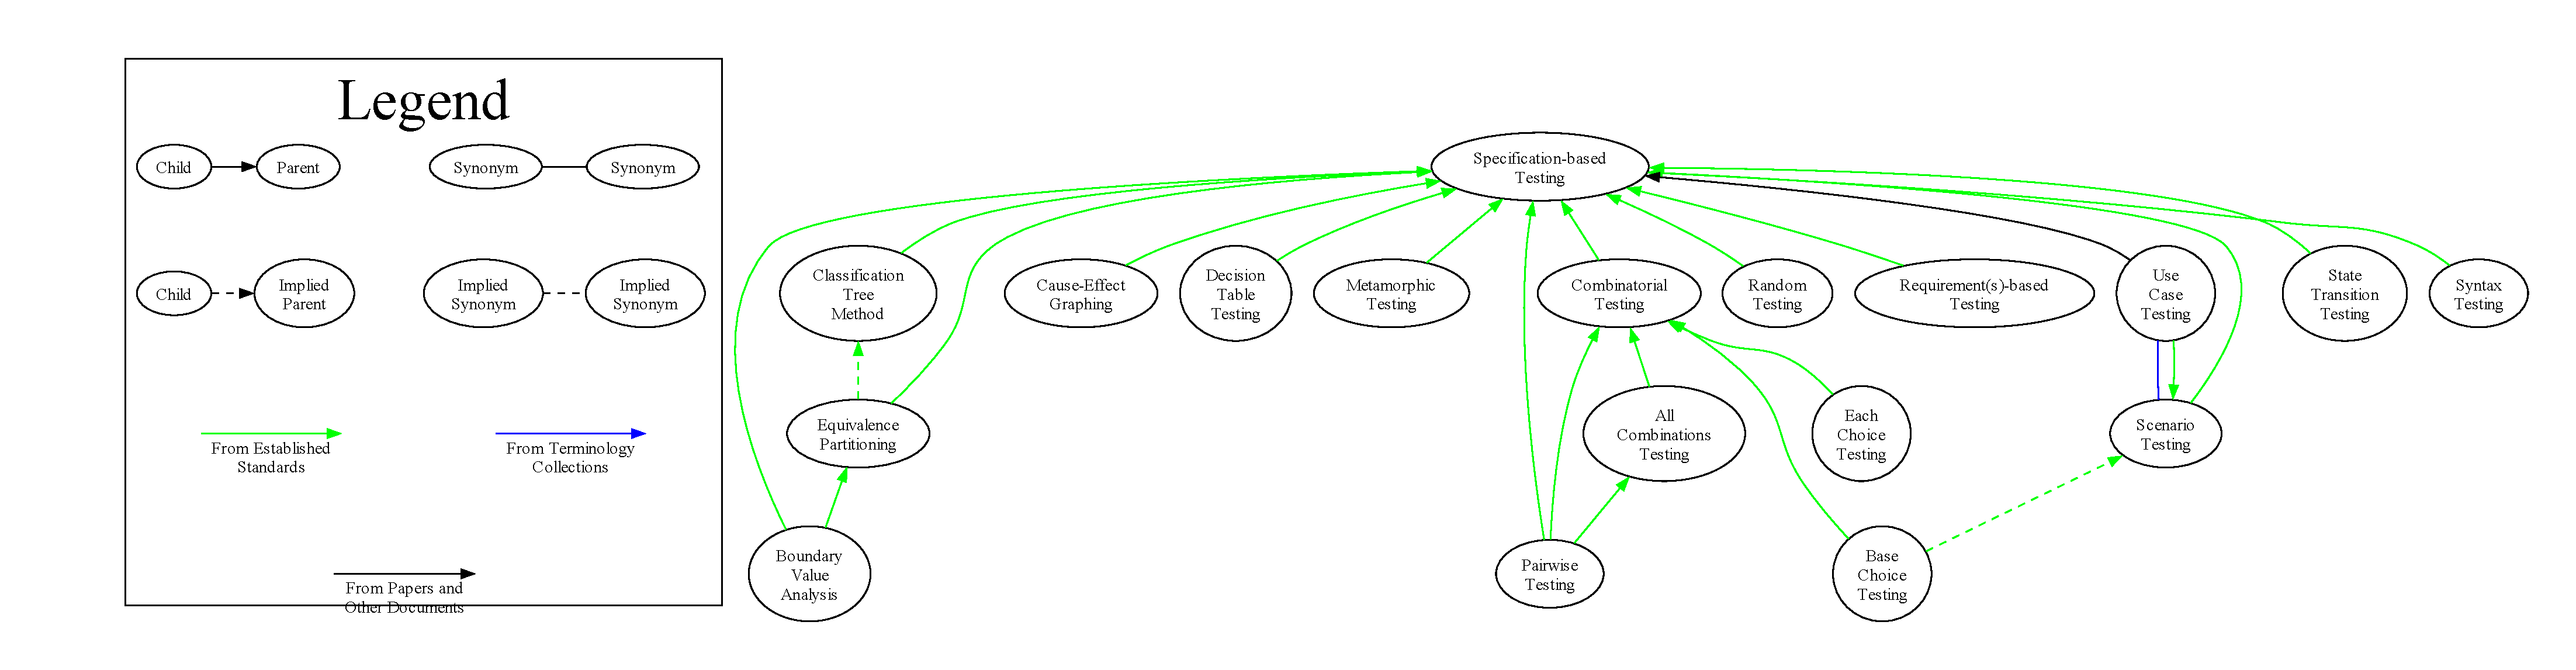
\includegraphics[width=\linewidth]{assets/graphs/specBasedGraph.pdf}
            \caption{``Superset'' relations.}
            \label{fig:specBasedGraph}
        \end{subfigure}
        \begin{subfigure}[t]{.45\linewidth}
            \centering
            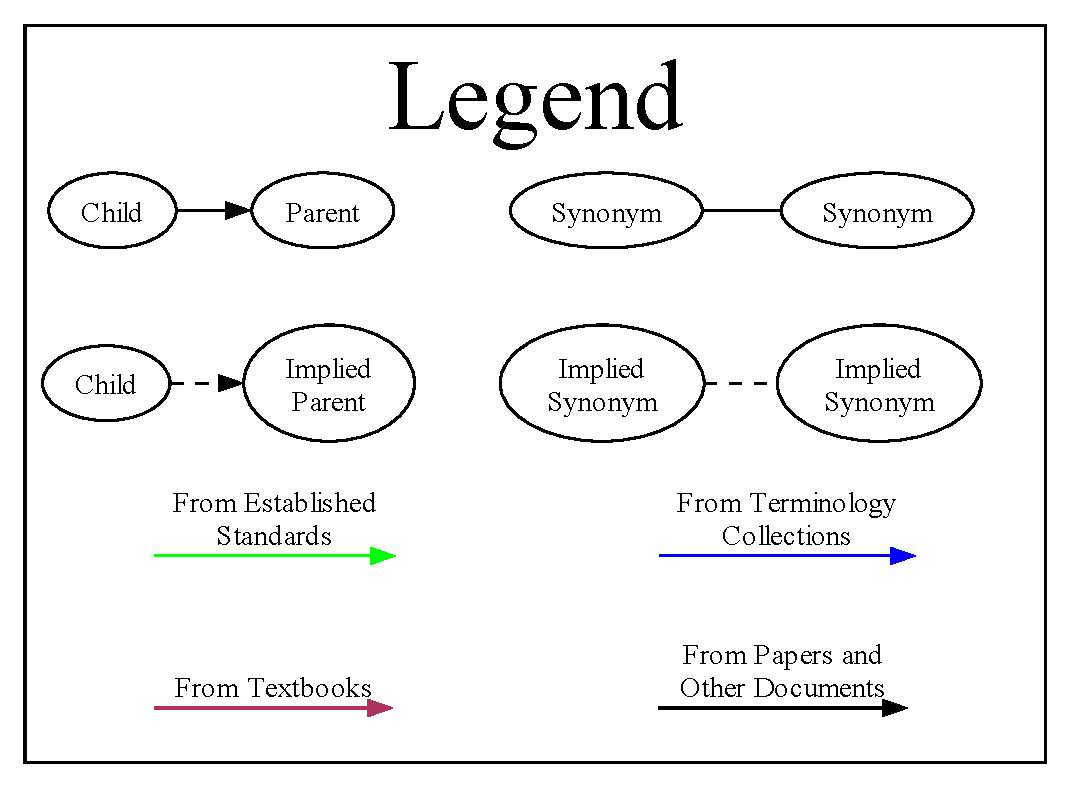
\includegraphics[width=\linewidth]{assets/graphs/parChdLegend.pdf}
        \end{subfigure}
        \begin{subfigure}[t]{.5\linewidth}
            \centering
            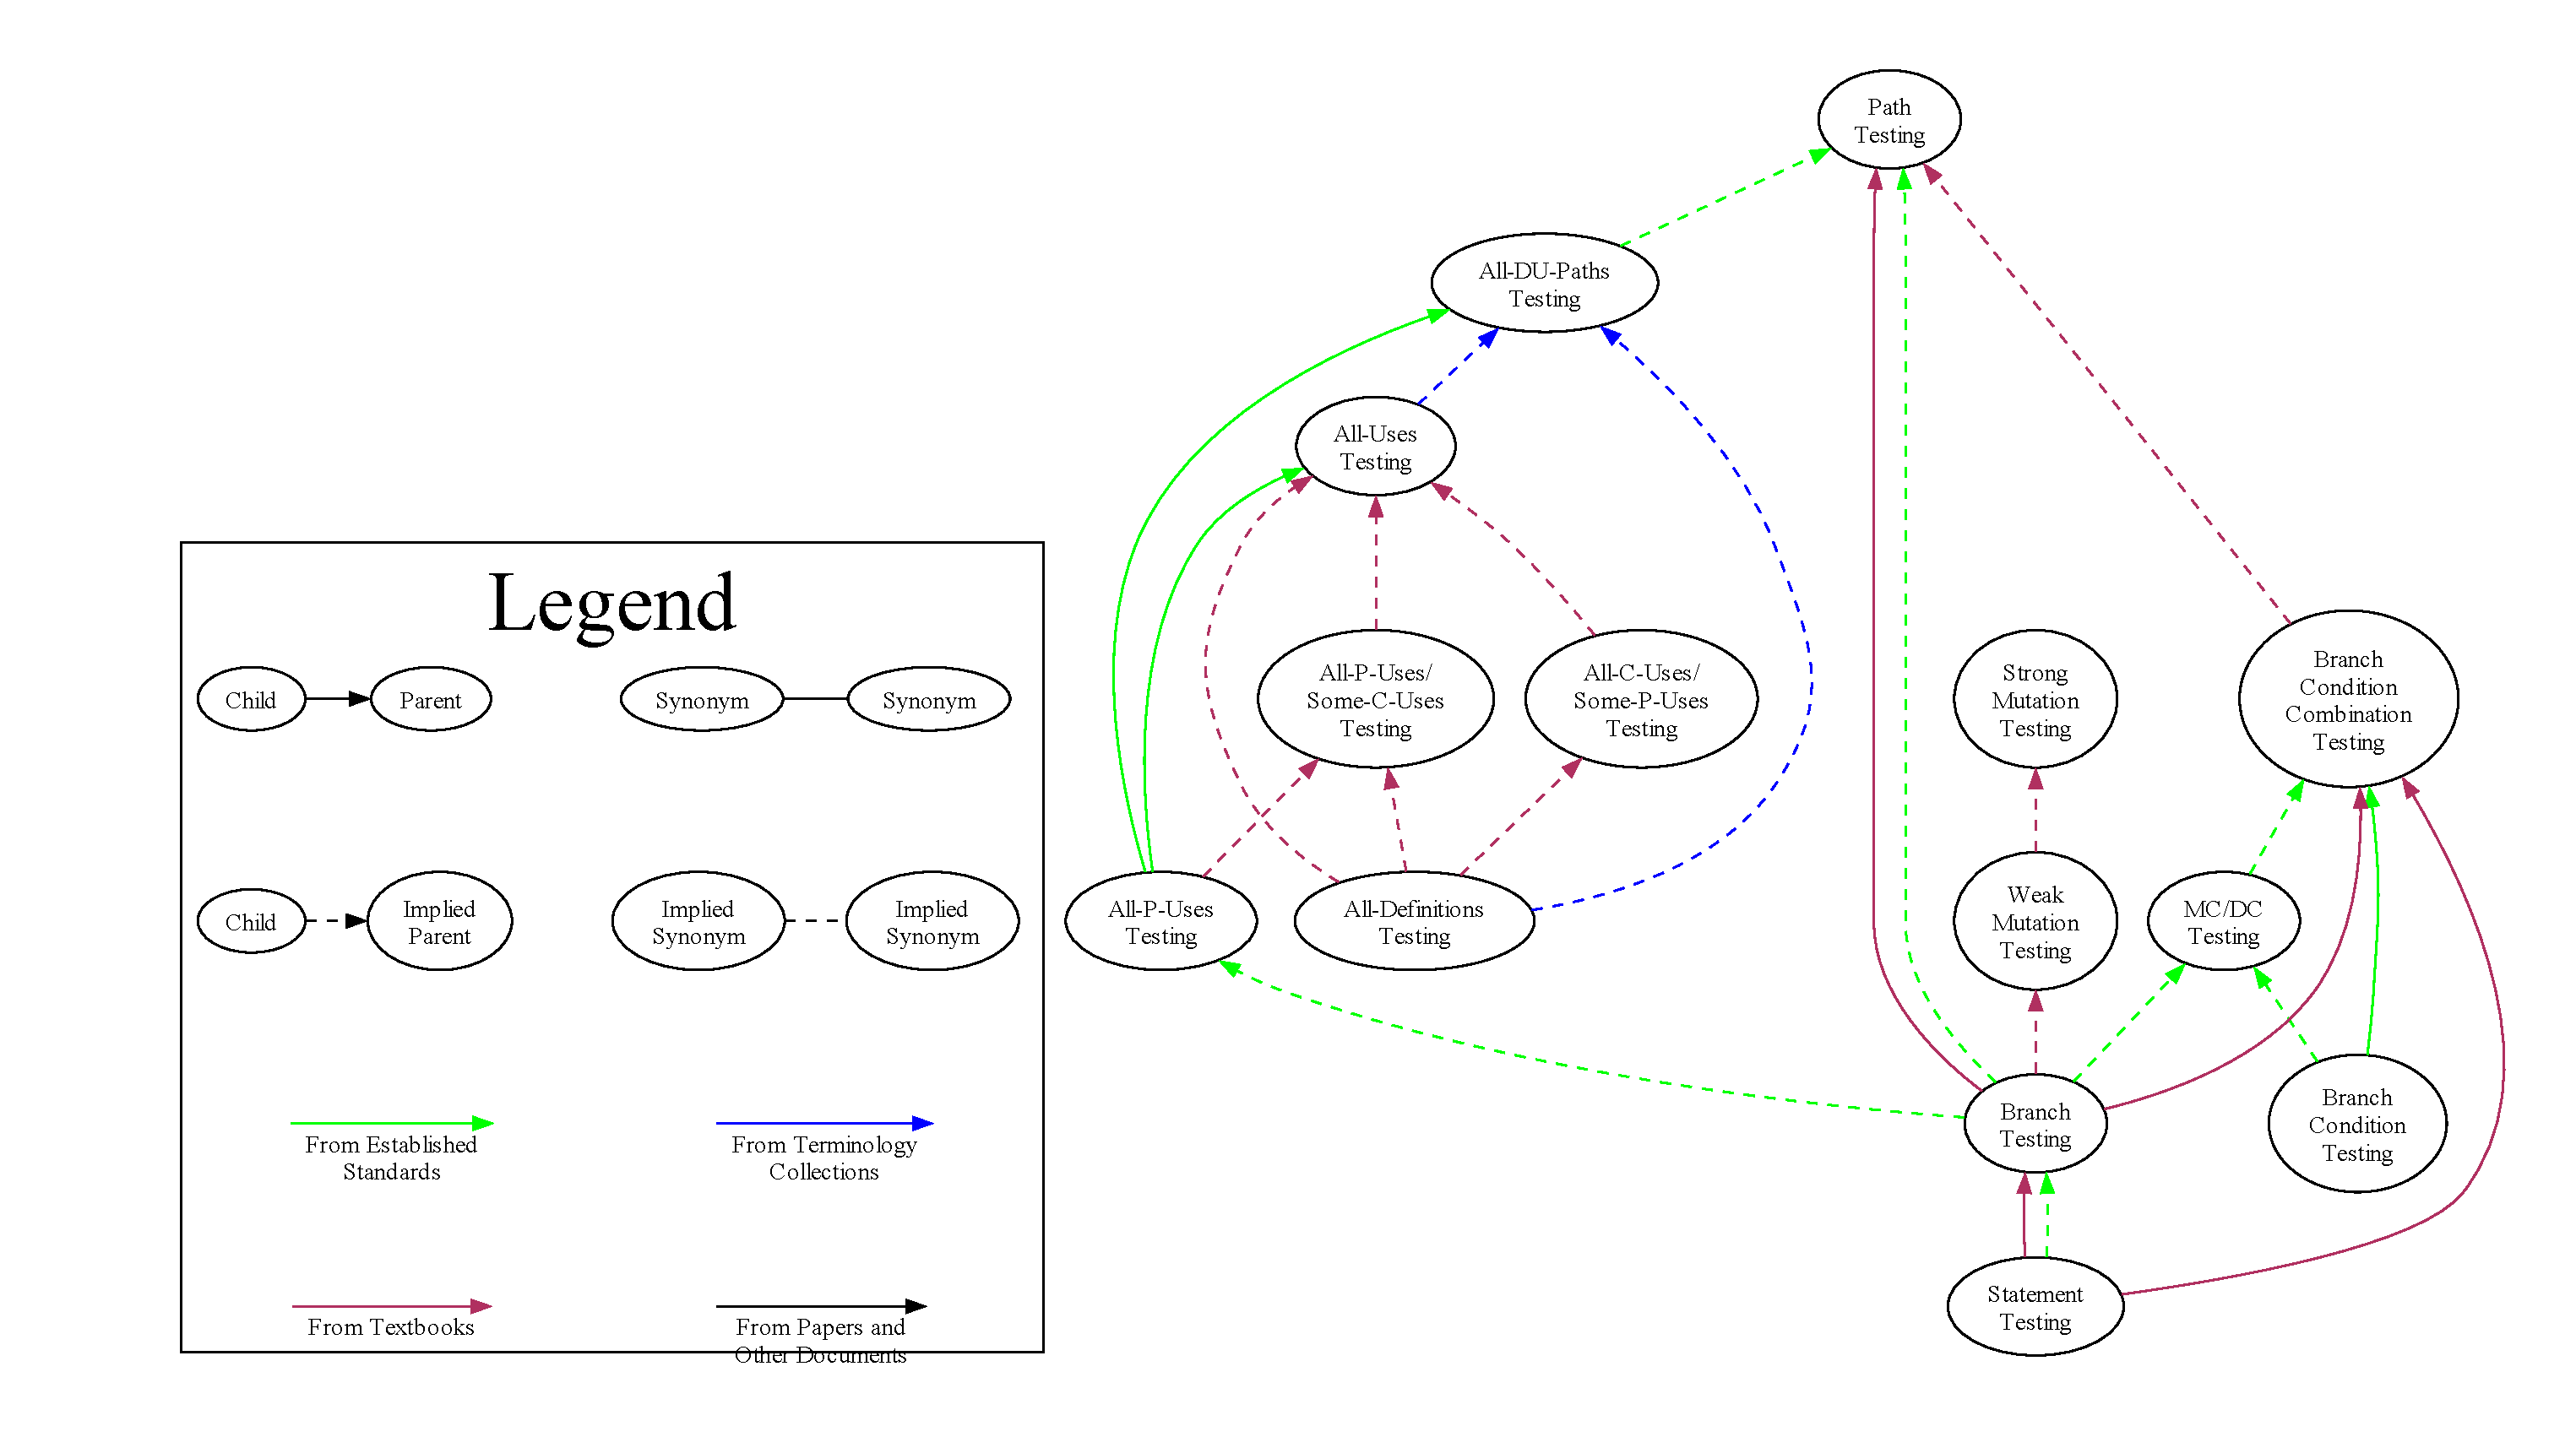
\includegraphics[width=\linewidth]{assets/graphs/subsumesGraph.pdf}
            \caption{``Subsume'' relations.}
            \label{fig:subsumesGraph}
        \end{subfigure}
        \caption{Graphs of different classes of \hyperref[par-chd-rels]{parent-child relations}.}
        \label{fig:parChdGraphs}
    \end{figure}
}

\newcommand{\ExampleGraph}{
    \begin{figure*}
        \begin{subfigure}[b]{0.3\linewidth}
            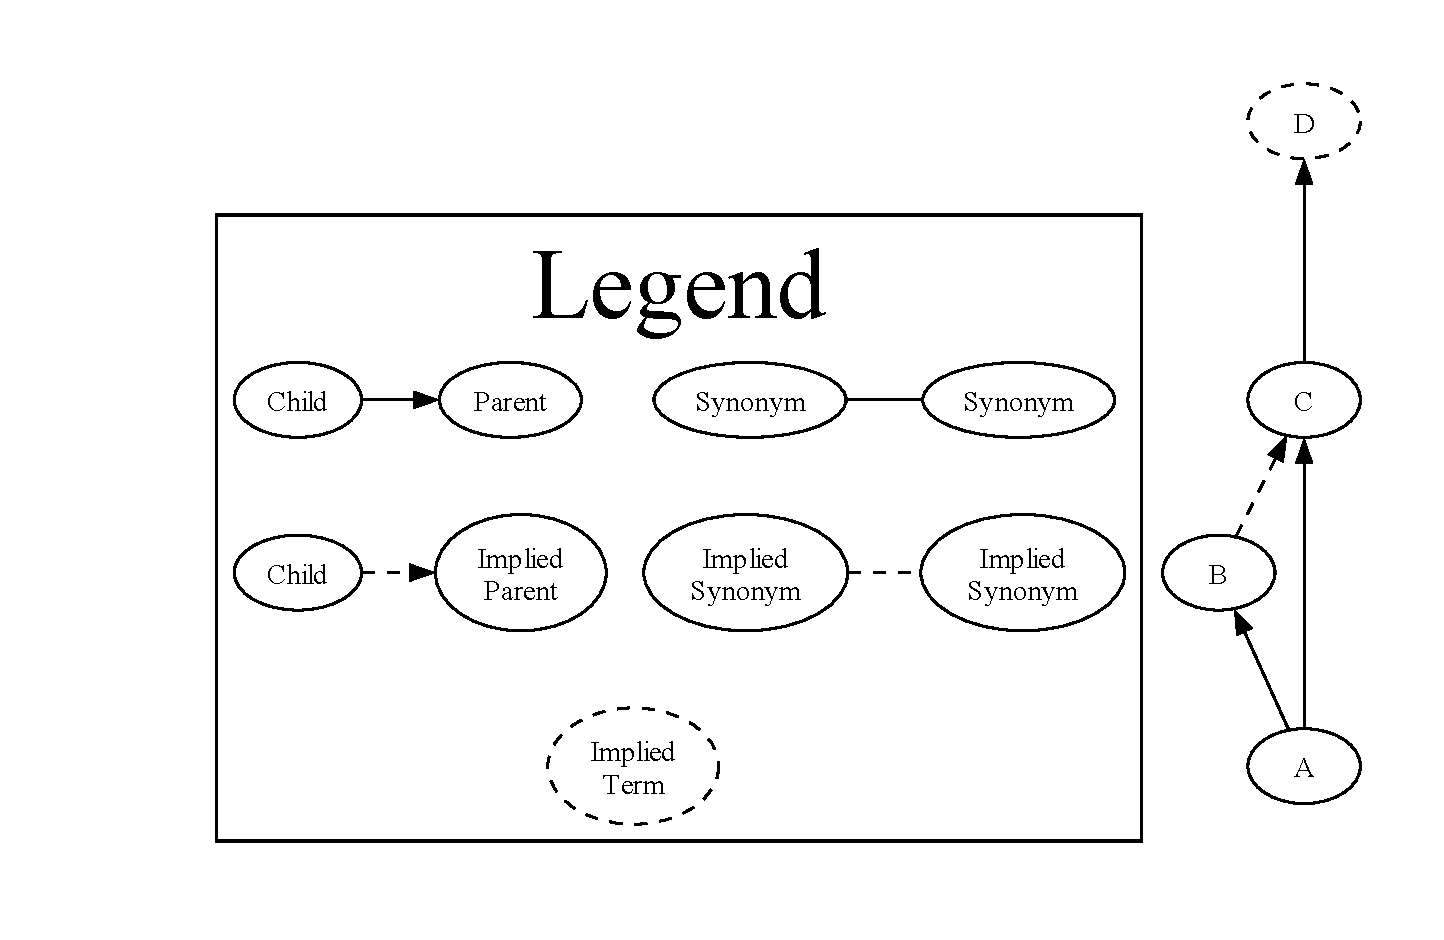
\includegraphics[width=\linewidth]{assets/graphs/ExampleGlossaryGraph.pdf}
            \caption{Graph from \Cref{tab:exampleGlossary}.}
            \label{fig:exampleGraph}
        \end{subfigure}
        \centering
        \begin{subfigure}[b]{0.675\linewidth}
            \centering
            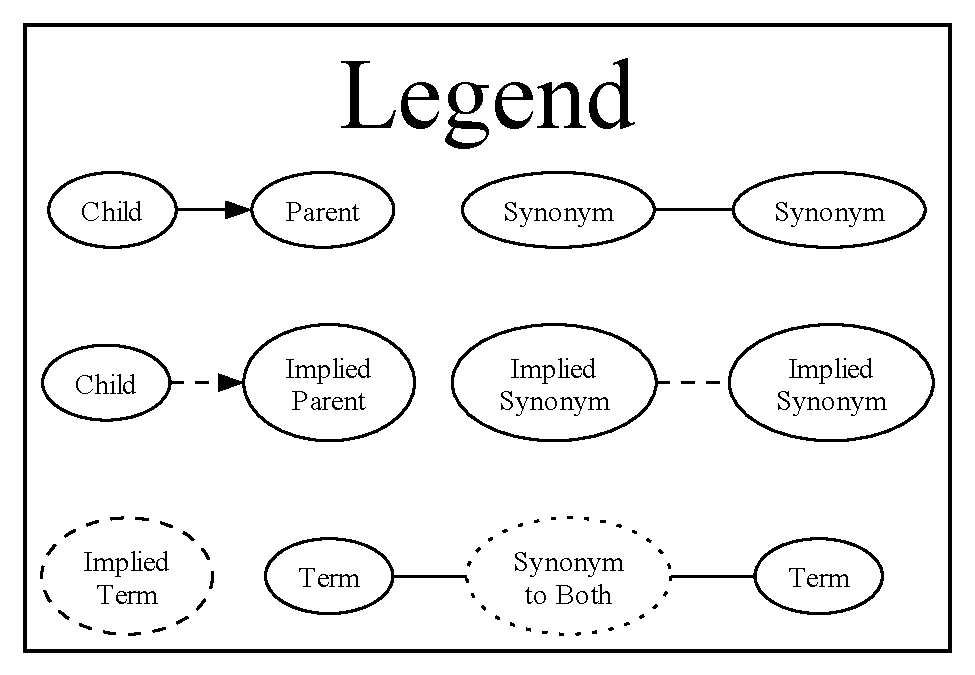
\includegraphics[width=0.8\linewidth]{assets/graphs/manual/manualLegendNonSolidTerms.pdf}
            \hspace{5cm}\begin{subfigure}[t]{0.475\linewidth}
                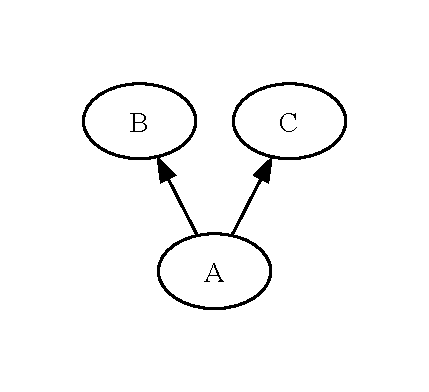
\includegraphics[width=1.1\linewidth]{assets/graphs/rigidExampleGlossaryGraph.pdf}
                \caption{Rigid graph from\\\Cref{tab:exampleGlossary}.}
                \label{fig:rigidExampleGraph}
            \end{subfigure}
            \begin{subfigure}[t]{0.475\linewidth}
                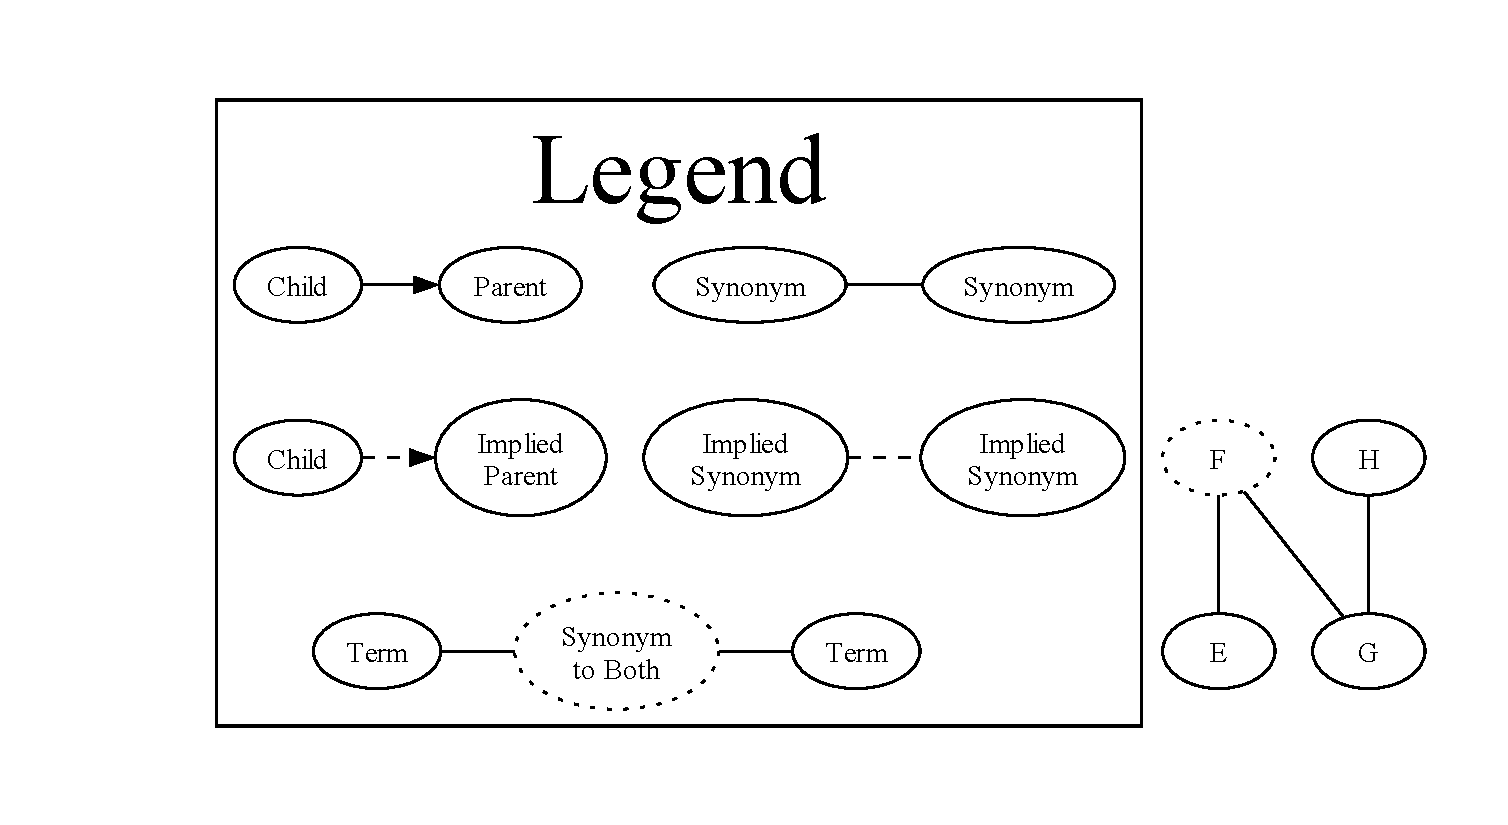
\includegraphics[width=1.1\linewidth]{assets/graphs/SynExampleGlossaryGraph.pdf}
                \caption{Graph from \Cref{tab:synExampleGlossary}.}
                \label{fig:synExampleGraph}
            \end{subfigure}
        \end{subfigure}
        \begin{subfigure}[t]{0.25\linewidth}
            \centering
            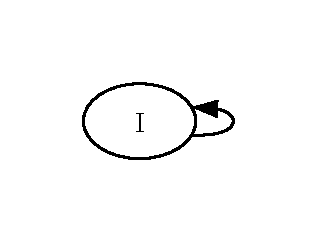
\includegraphics[width=1.2\linewidth]{assets/graphs/SelfExampleGlossaryGraph.pdf}
            \caption{Self-loop graph.}
            \label{fig:selfExampleGraph}
        \end{subfigure}
        \hfill
        \begin{subfigure}[t]{0.425\linewidth}
            \centering
            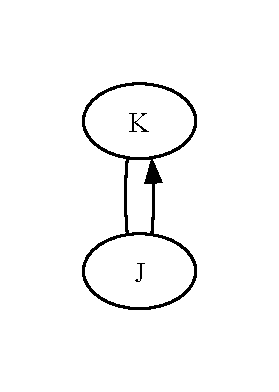
\includegraphics[width=0.6\linewidth]{assets/graphs/ParSynExampleGlossaryGraph.pdf}
            \caption{Graph of a pair of terms with a \hyperref[par-chd-rels]{parent-child} \emph{and} synonym relation.}
            \label{fig:parSynExampleGraph}
        \end{subfigure}
        \hfill
        \begin{subfigure}[t]{0.25\linewidth}
            \centering
            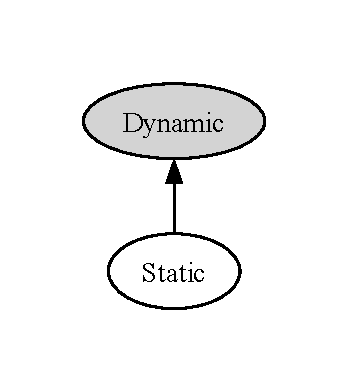
\includegraphics[width=1.4\linewidth]{assets/graphs/StaticExampleGlossaryGraph.pdf}
            \caption{Static graph.}
            \label{fig:staticExampleGraph}
        \end{subfigure}
        \caption{Example generated graphs.}
        \label{fig:exampleGraphs}
    \end{figure*}
}

\newcommand{\recoveryGraphs}{
    % Only top or bottom to comply with IEEE guidelines
    \begin{figure}[bt!]
        \centering
        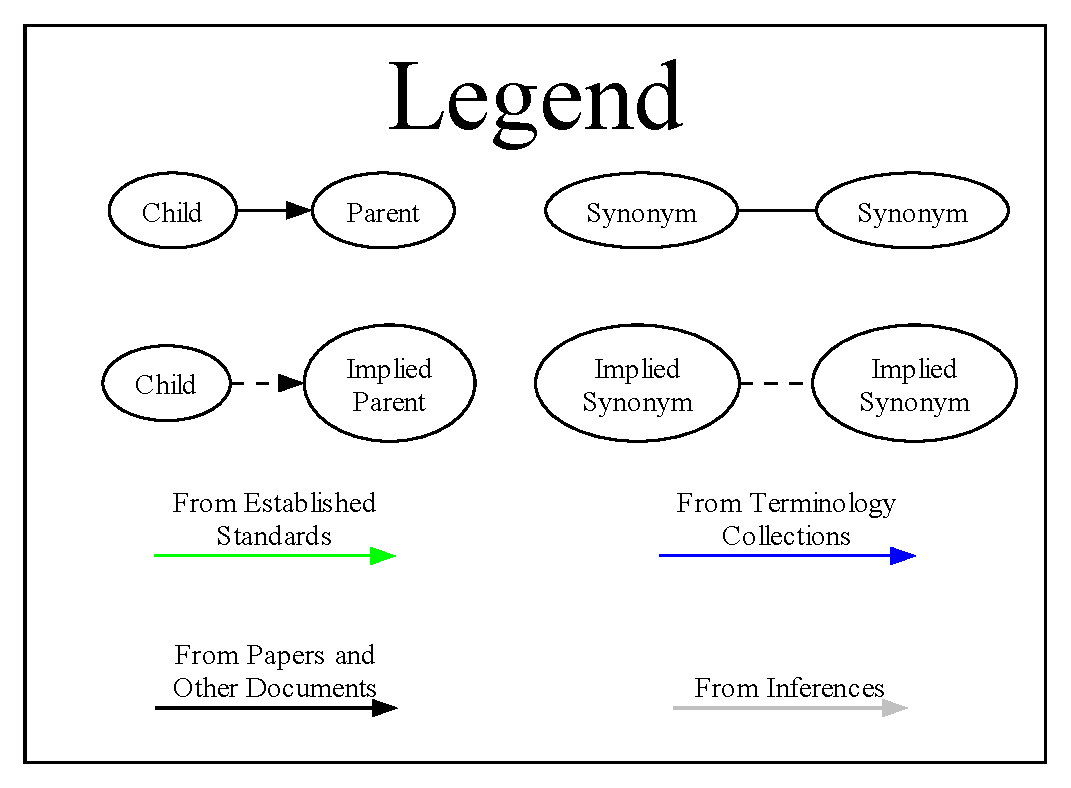
\includegraphics[width=\linewidth]{assets/graphs/recoveryLegend.pdf}
        \begin{subfigure}[b]{.55\linewidth}
            \centering
            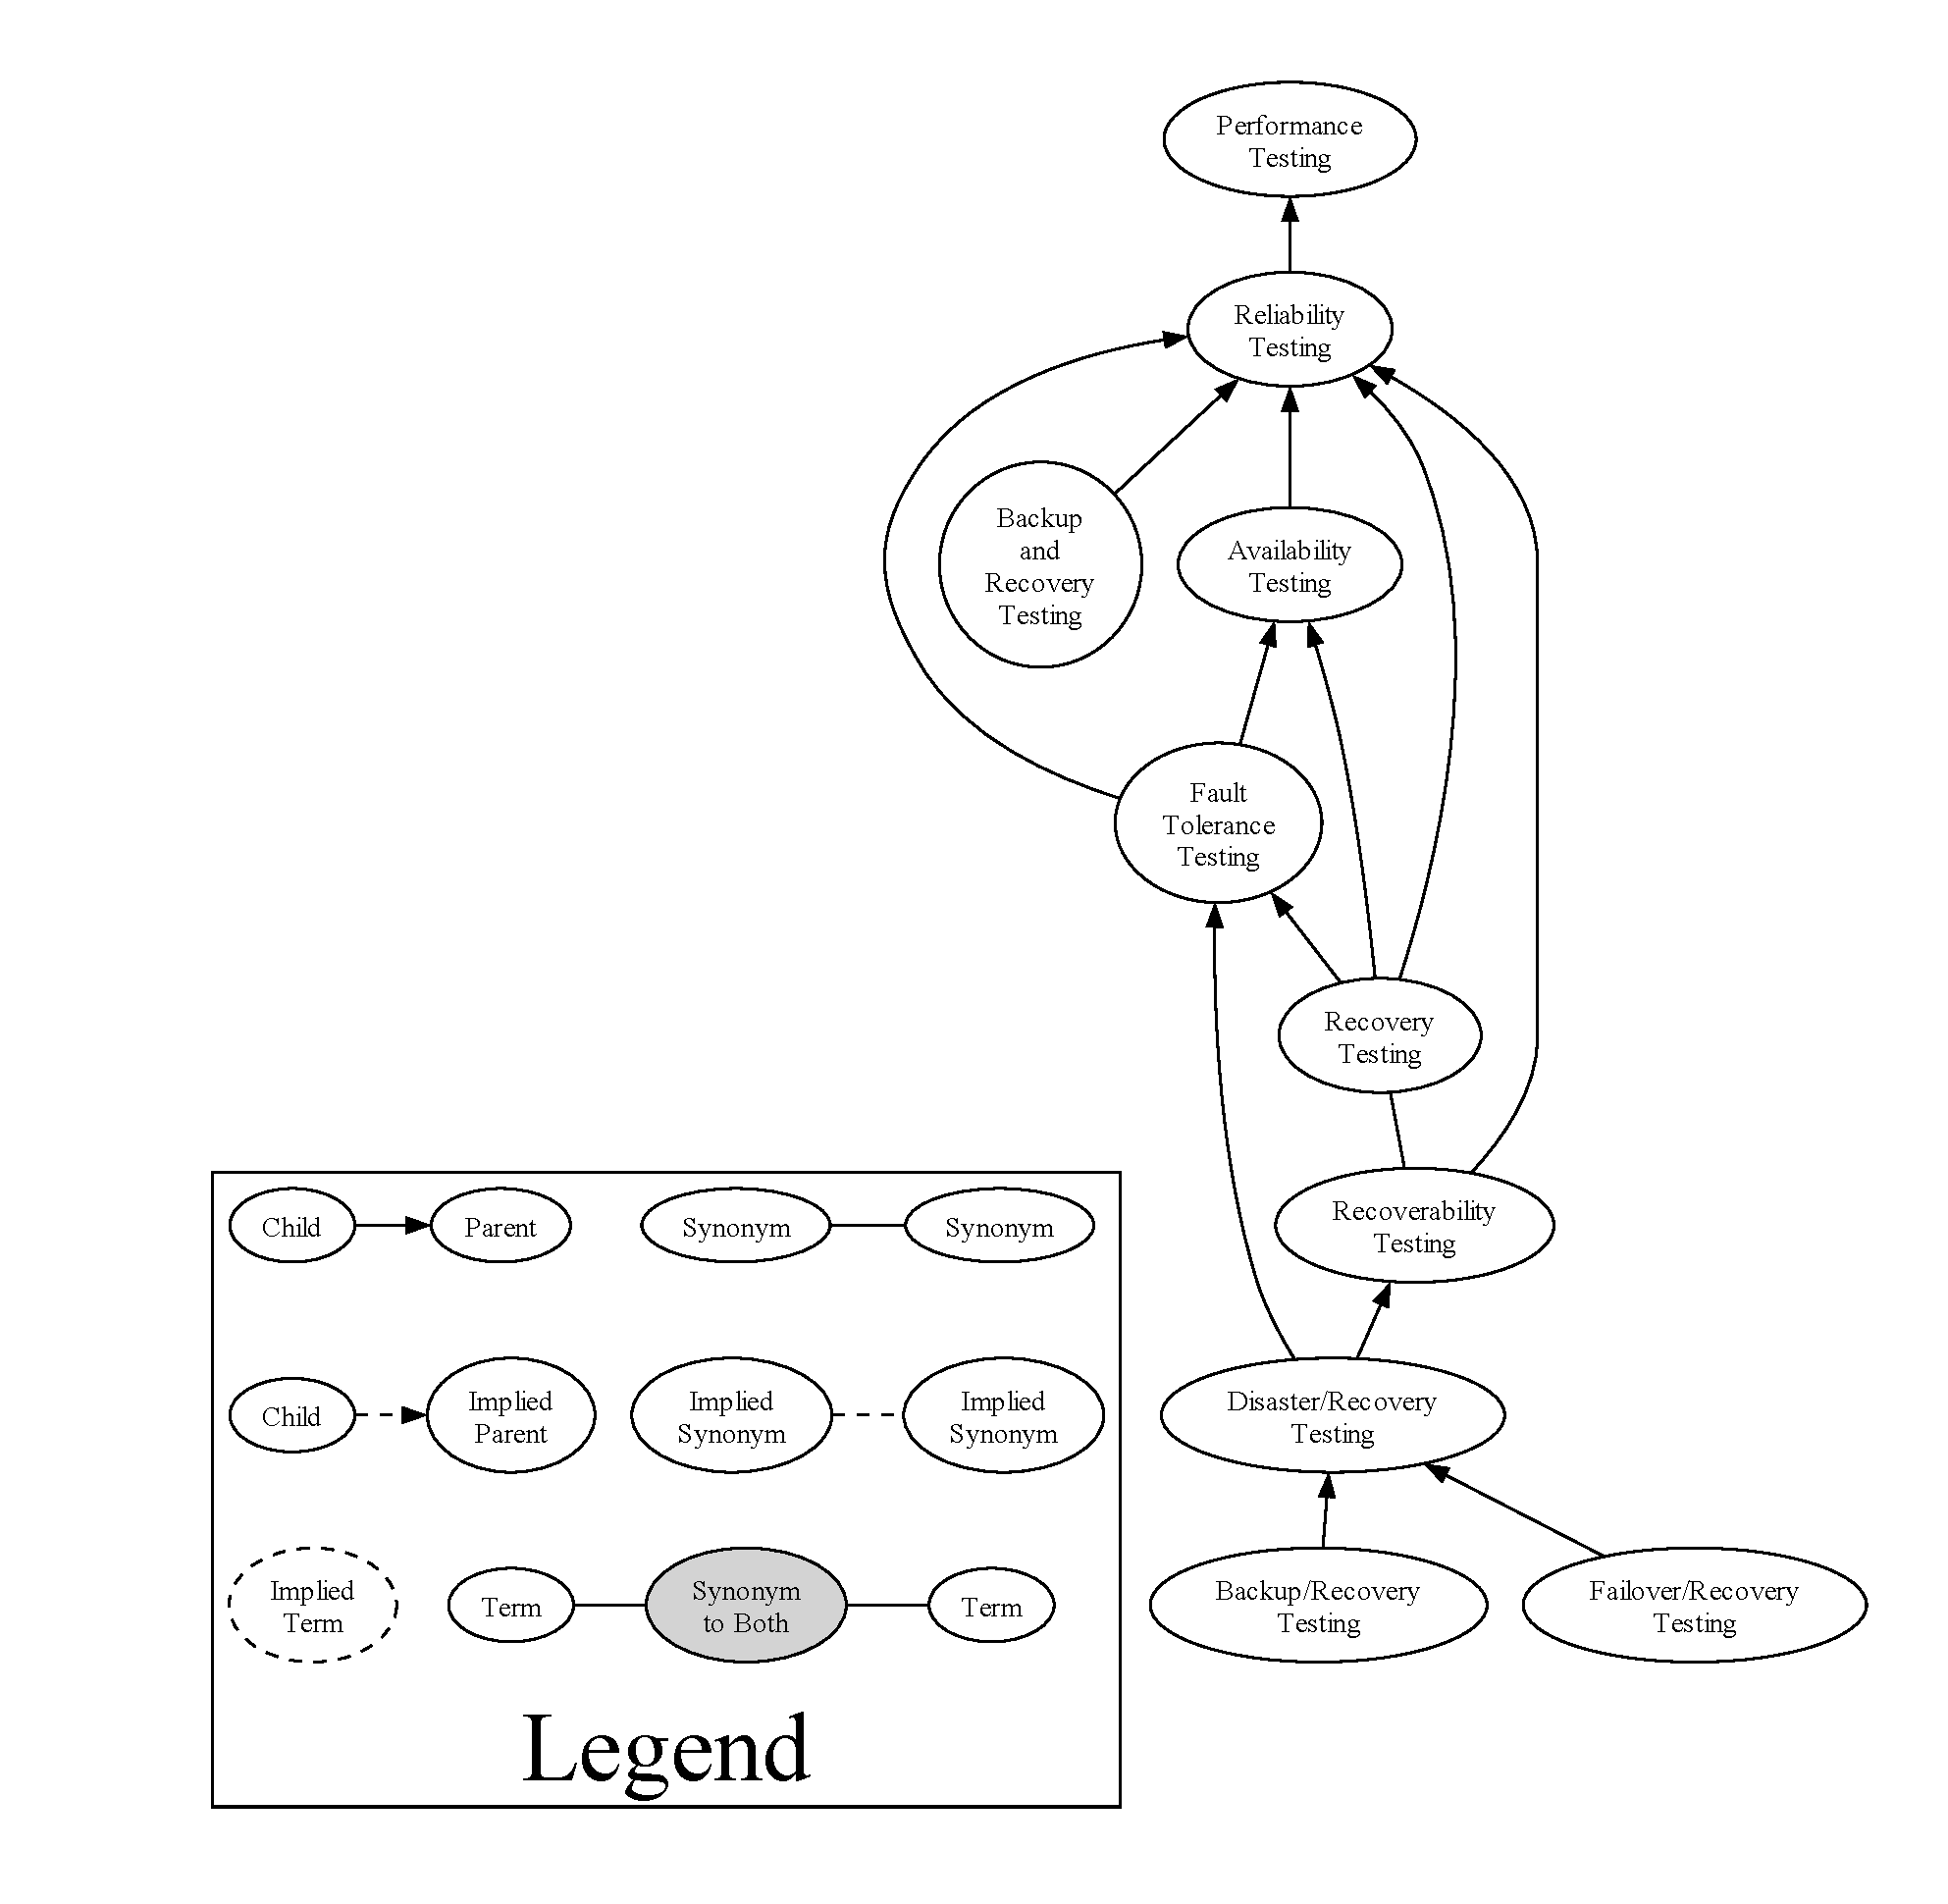
\includegraphics[width=\linewidth]{assets/graphs/recoveryGraph.pdf}
            \caption{Graph of current relations.}
            \label{fig:recovery-graph-current}
        \end{subfigure}
        \begin{subfigure}[b]{.4\linewidth}
            \centering
            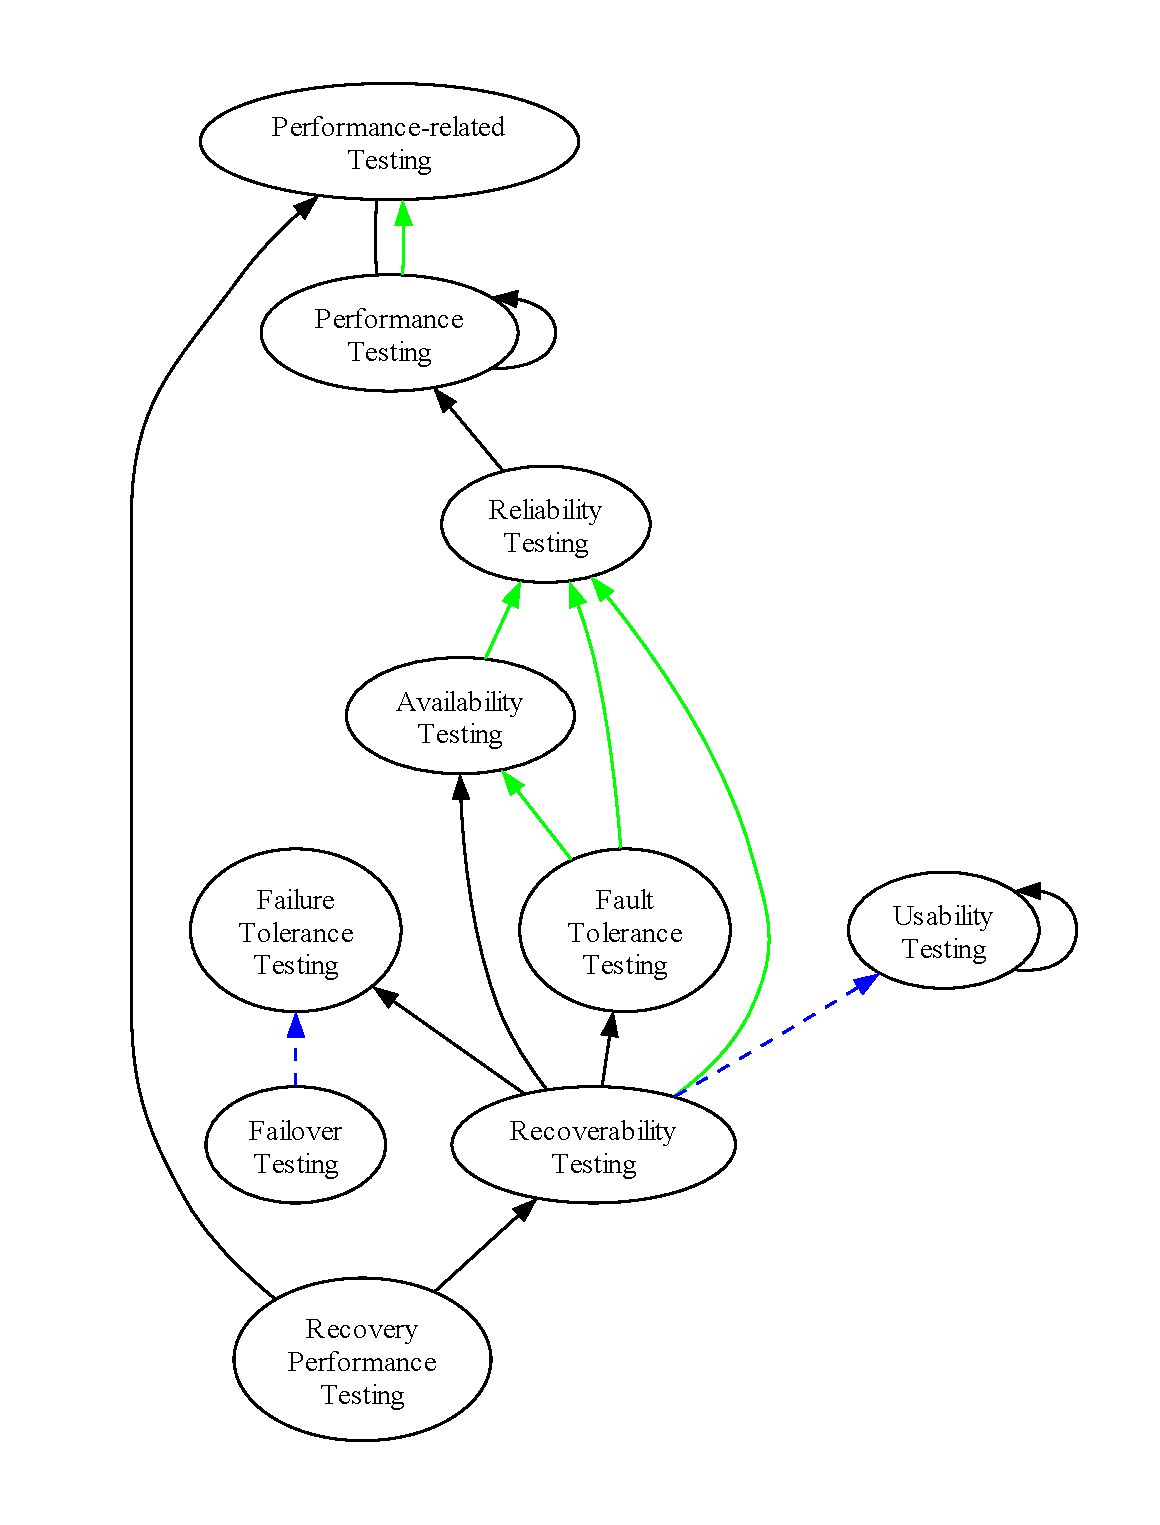
\includegraphics[width=\linewidth]{assets/graphs/recoveryProposedGraph.pdf}
            \caption{Graph of proposed relations.}
            \label{fig:recovery-graph-proposed}
        \end{subfigure}
        \caption{Graphs of relations between terms related to recovery testing.}
        \label{fig:recoveryGraphs}
    \end{figure}
}

\newcommand{\scalGraphs}{
    % Only top or bottom to comply with IEEE guidelines
    \begin{figure}[bt!]
        \centering
        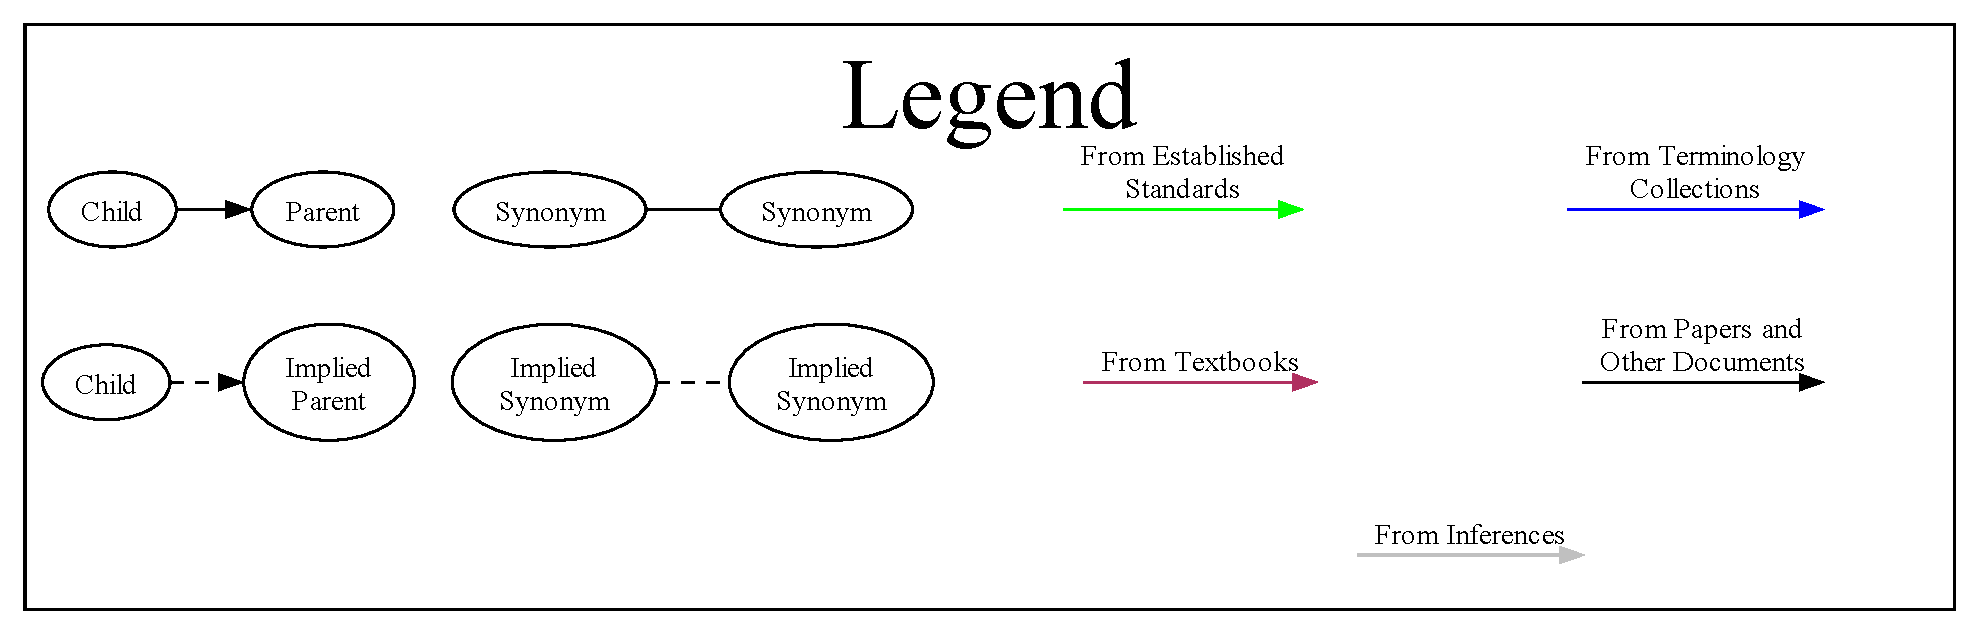
\includegraphics[width=\linewidth]{assets/graphs/scalabilityLegend.pdf}
        \begin{subfigure}[b]{.475\linewidth}
            \centering
            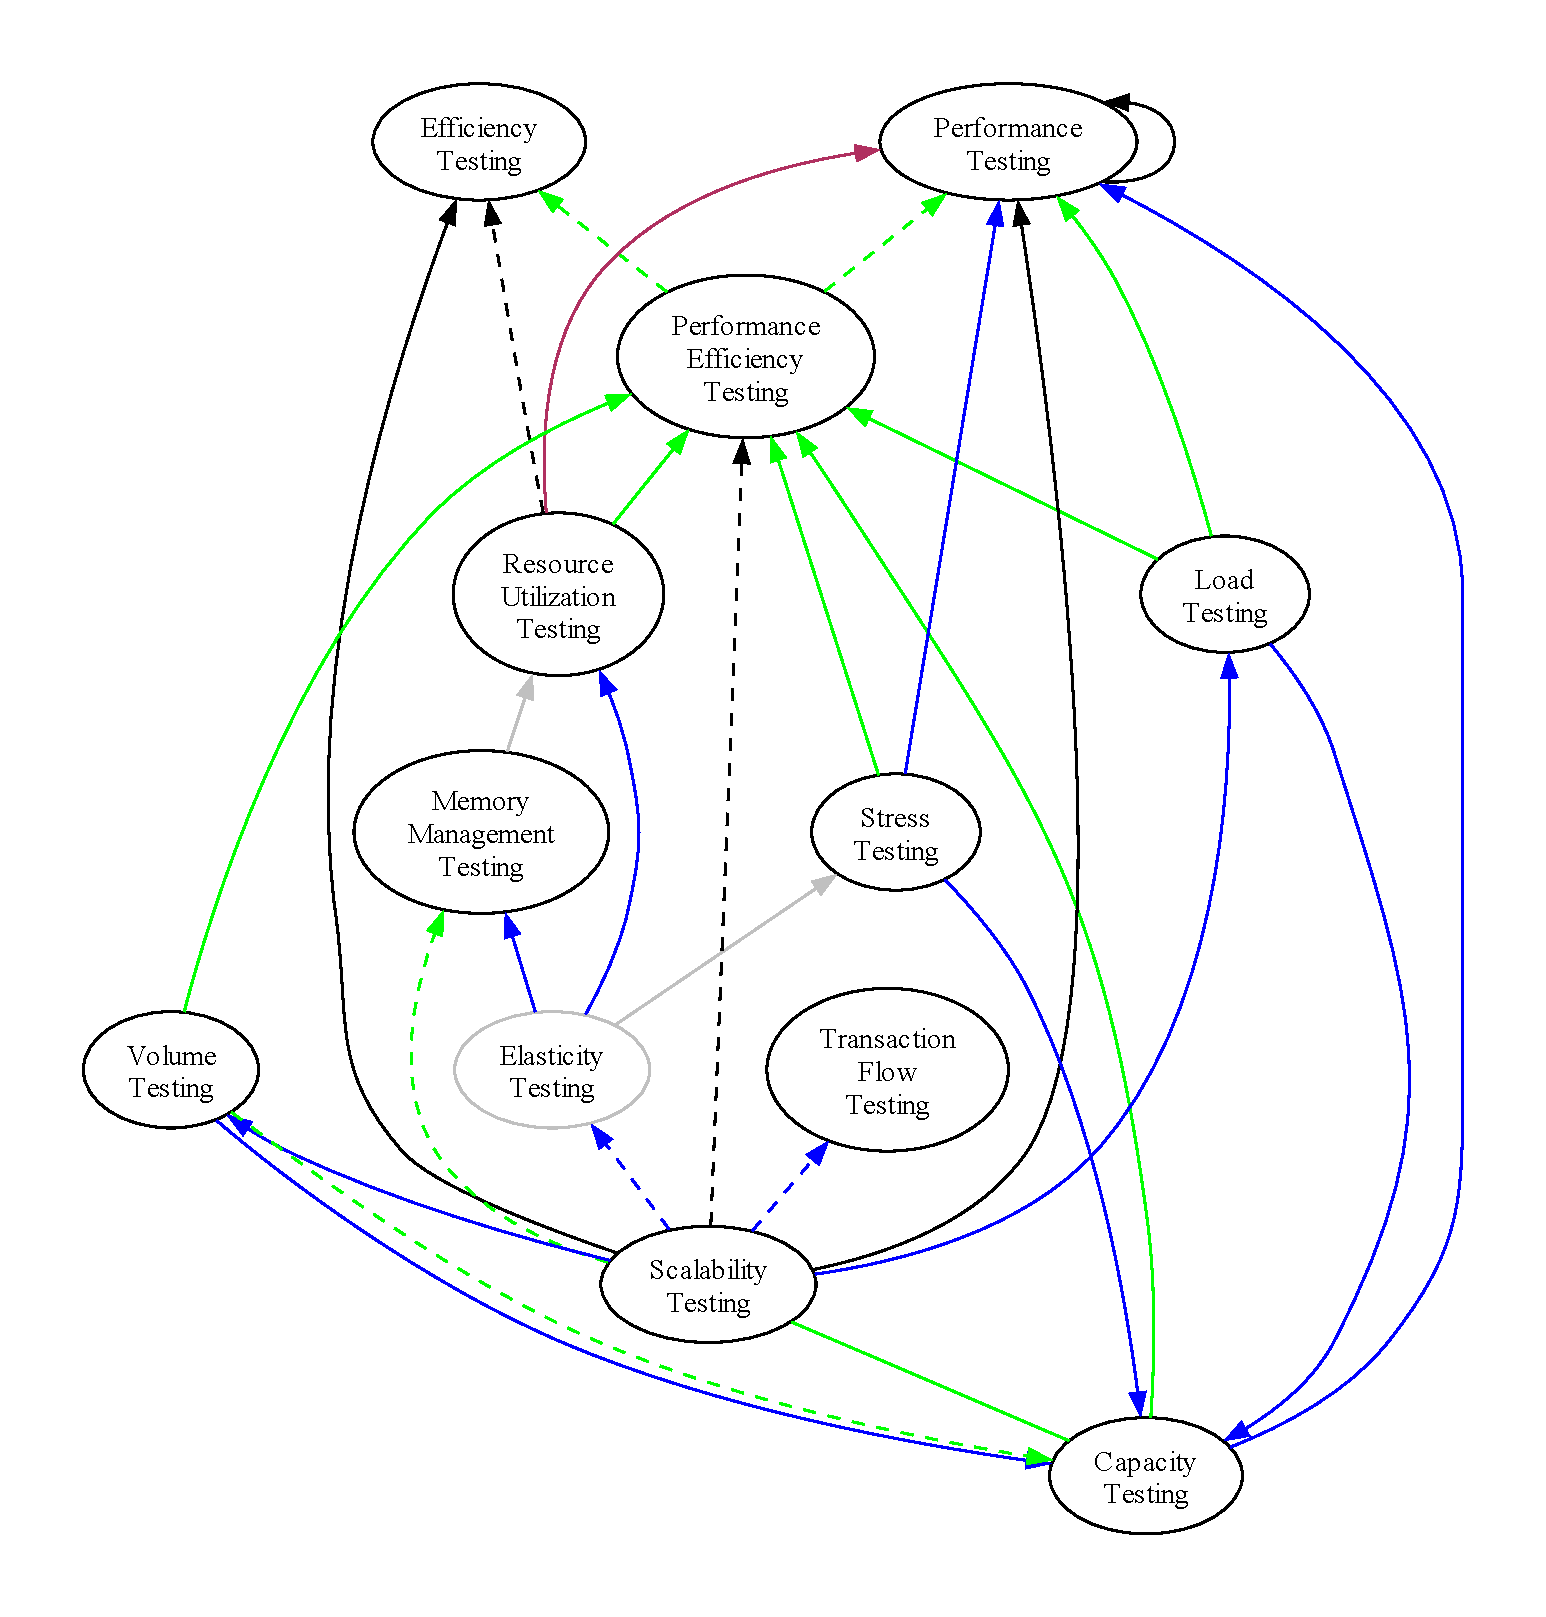
\includegraphics[width=\linewidth]{assets/graphs/scalabilityGraph.pdf}
            \caption{Graph of current relations.}
            \label{fig:scal-graph-current}
        \end{subfigure}
        \begin{subfigure}[b]{.475\linewidth}
            \centering
            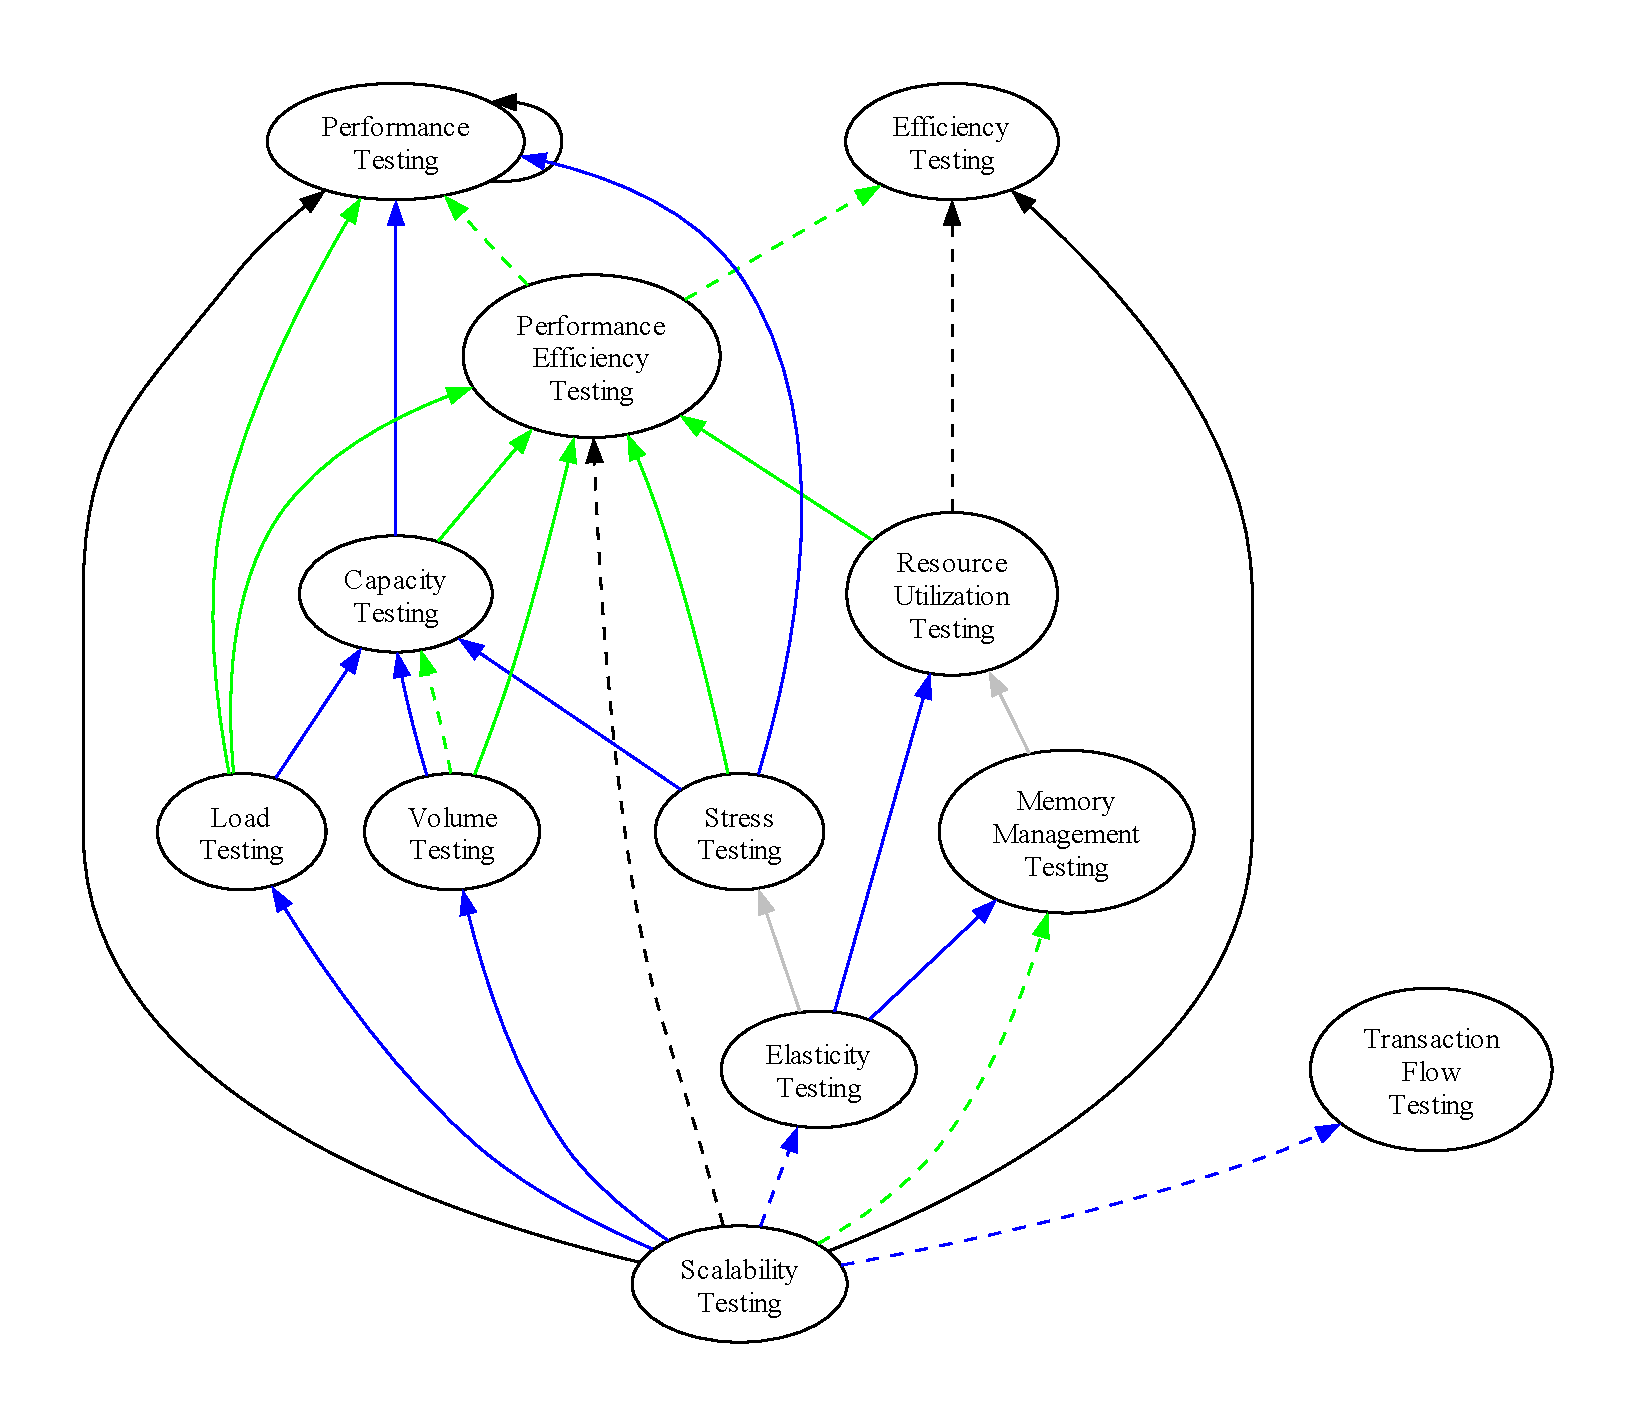
\includegraphics[width=\linewidth]{assets/graphs/scalabilityProposedGraph.pdf}
            \caption{Graph of proposed \ifnotpaper \else \\ \fi relations.}
            \label{fig:scal-graph-proposed}
        \end{subfigure}
        \caption{Graphs of relations between terms related to scalability testing.}
        \label{fig:scalGraphs}
    \end{figure}
}

\newcommand{\performanceGraph}{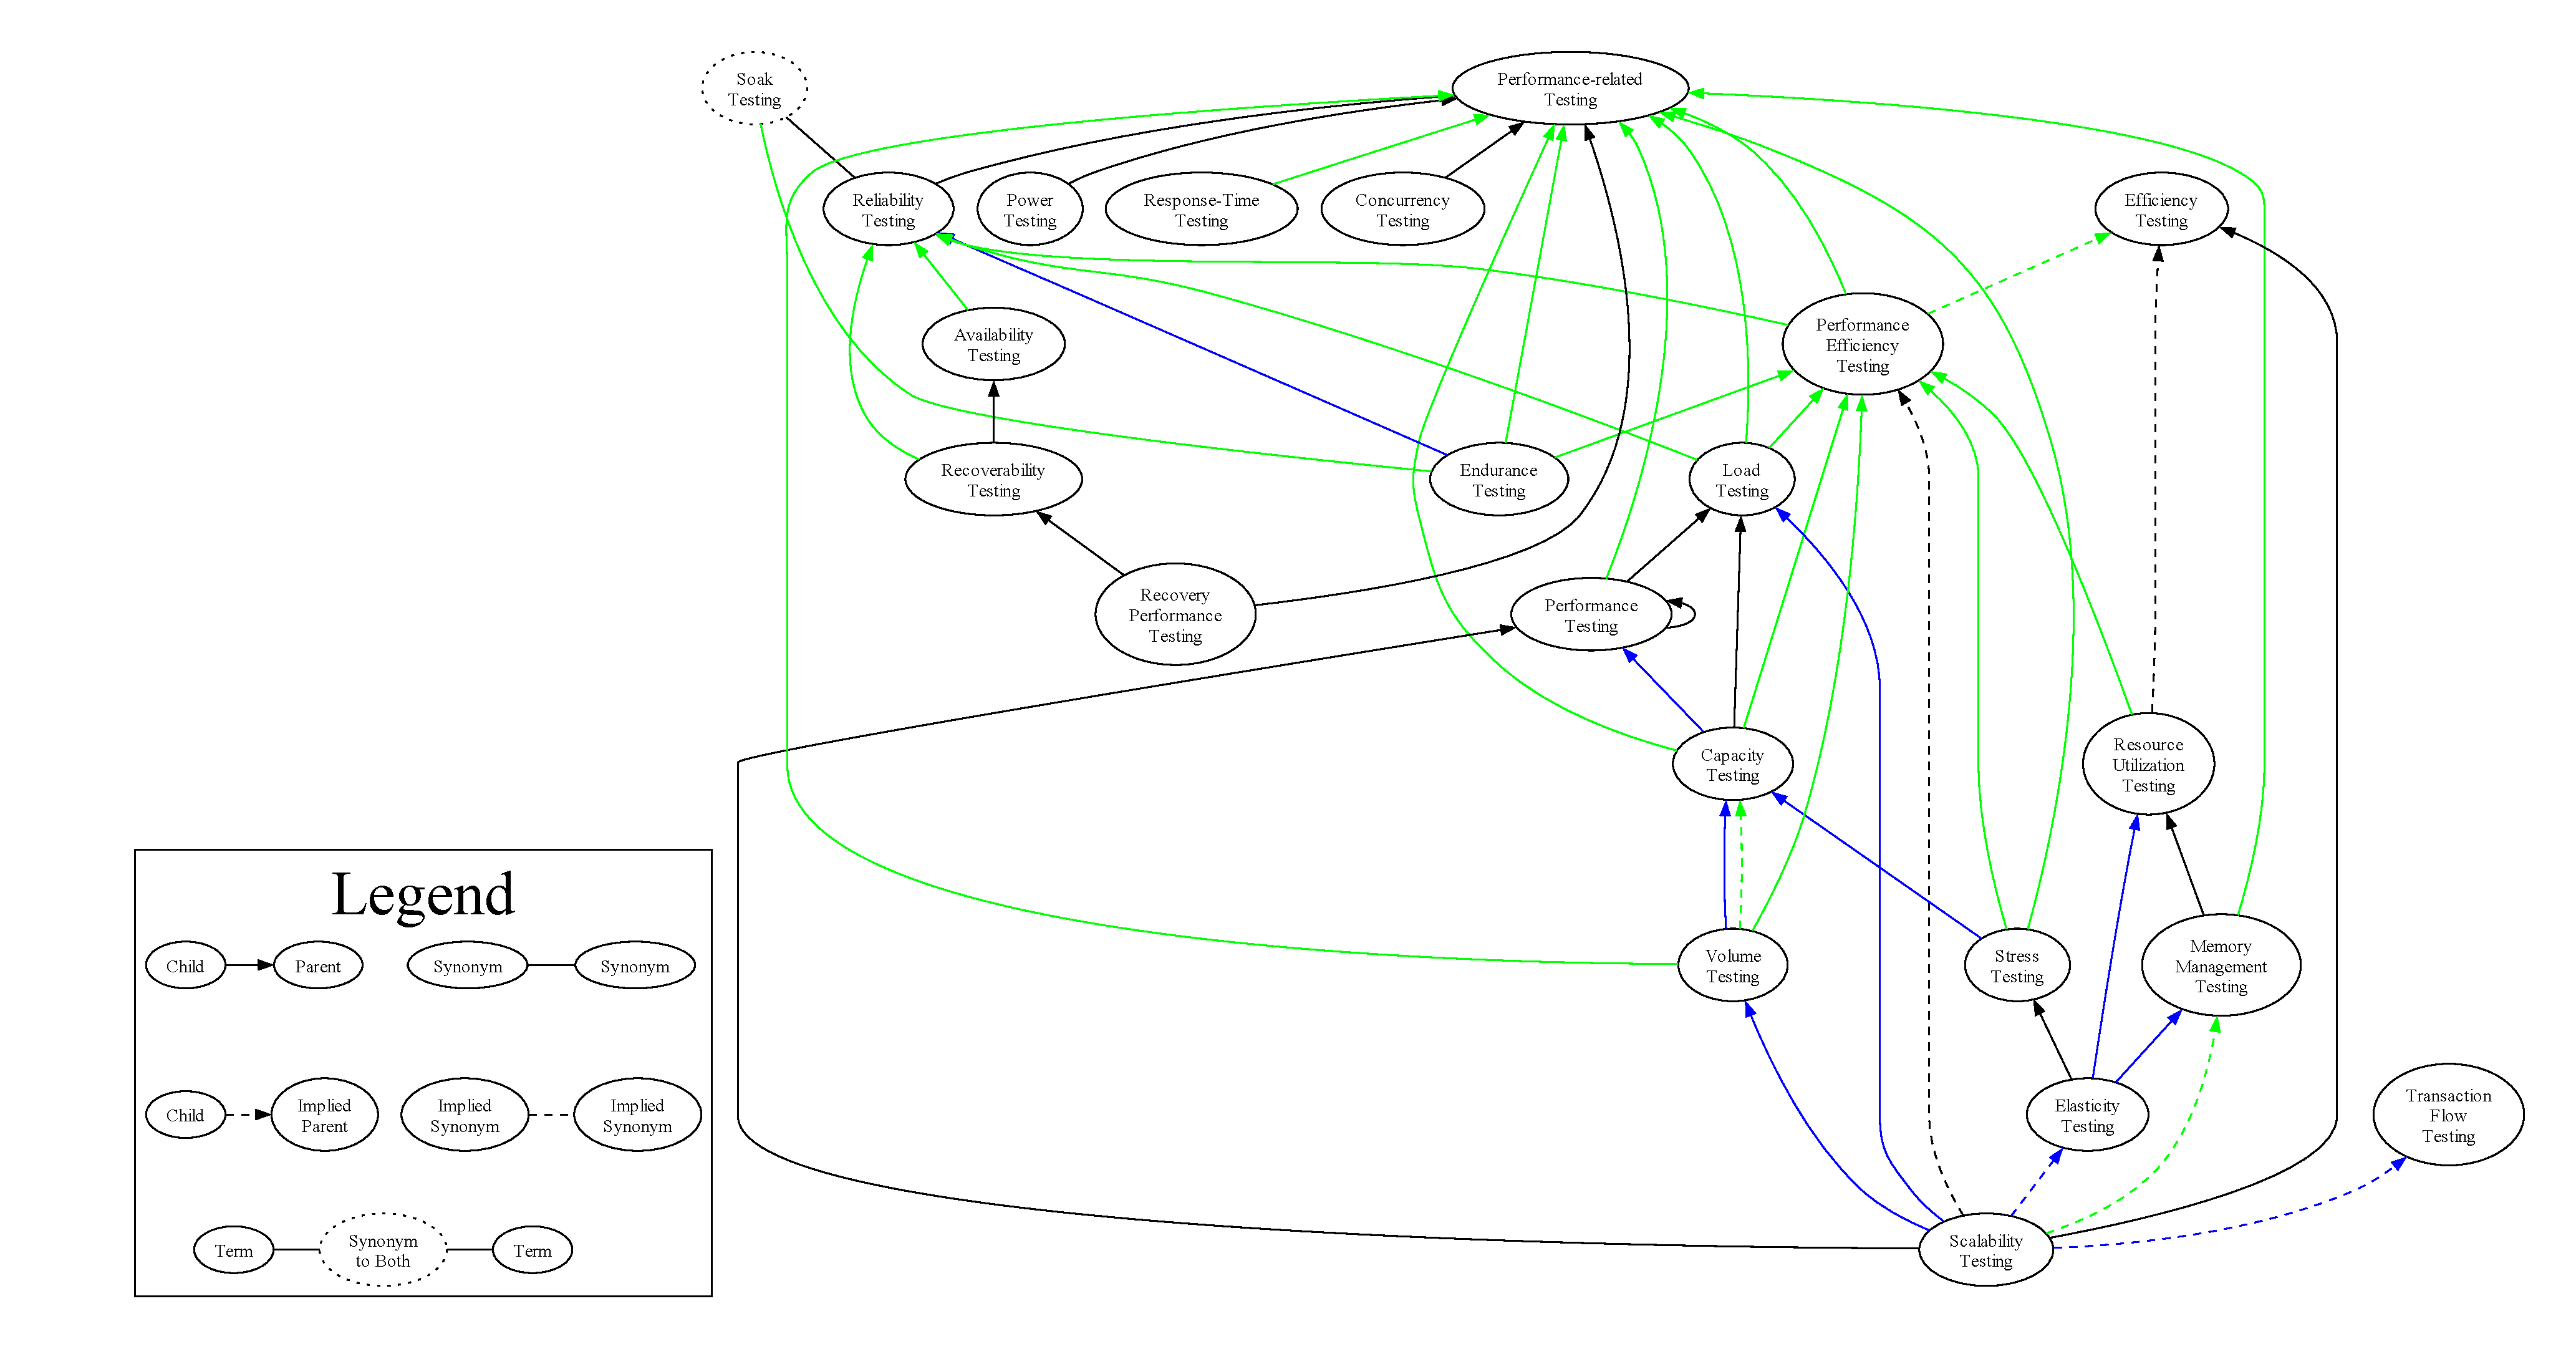
\includegraphics[width=\linewidth]{assets/graphs/performanceProposedGraph.pdf}}

%------------------------------------------------------------------------------
% Images & Figures
%------------------------------------------------------------------------------

\newcommand{\drasilLogo}{assets/images/drasil_logo.png}
\newcommand{\drasilLogoImg}{\input{assets/images/drasil_logo}}
\newcommand{\refDrasilLogoImg}{\Cref{fig:drasilLogo}}

%------------------------------------------------------------------------------
% Tables
%------------------------------------------------------------------------------

% Organization of files
\newcommand{\organizationTable}{\input{assets/tables/organization}}

\newcommand{\ieeeCatsTable}{\input{assets/tables/ieeeCats}}
\newcommand{\otherCatsTable}{\input{assets/tables/otherCats}}
\newcommand{\otherCategorizationsTable}{\input{assets/tables/otherCategorizations}}

\newcommand{\sntxFlawsTable}{\input{assets/tables/sntxFlaws}}
\newcommand{\smntcFlawsTable}{\input{assets/tables/smntcFlaws}}

\newcommand{\testReqsTable}{\input{assets/tables/testReqs}}


% Enable links within the document
\usepackage{hyperref}
\hypersetup{
    linkcolor=red,
    urlcolor=red,
    breaklinks=true,
    pdftitle={\thesisTitle{}},
}
\urlstyle{rm} % Make URL styled fonts match hyperref's hrefs
\usepackage[capitalize]{cleveref} % Fixes capitalization of internal references

% General Utility Functions
\def\sWidth{3.4cm}
\def\tWidth{0.7cm}
% Extra functionality for command parsing
\usepackage{xparse}

\newif\ifnotpaper

%------------------------------------------------------------------------------
% Reused in seminar slides
%------------------------------------------------------------------------------

\def\rqatext{What testing approaches do the literature describe?}
\def\rqbtext{Are these descriptions consistent?}
\def\rqctext{Can we systematically resolve any of these inconsistencies?}

\def\expBasedCatMain{\citeauthor{IEEE2022} categorize experience-based testing
    as both a test design technique and a test practice on the same
    page---twice \citeyearpar[Fig.~2, p.~34]{IEEE2022}!}

\NewDocumentCommand{\perfAsFamily}{s}{%
    \IfBooleanTF#1{\citealp}{\citep}[p.~1187]{Moghadam2019}\footnote{
        The original source describes ``performance testing \dots\ as a family
        of performance-related testing techniques'', but it makes more sense to
        consider ``performance-related testing'' as the ``family'' with
        ``performance testing'' being one of the variabilities
        (see \Cref{perf-test-rec}).}%
}

\def\supersAck{Drs.~Spencer Smith and Jacques Carette have been great
    supervisors in the past and have, both then and now, provided me
    with valuable guidance and feedback}

%------------------------------------------------------------------------------
% Spacing Options
%------------------------------------------------------------------------------

\newcommand{\thesisForceSingleSpacing}{\singlespacing}
\newcommand{\thesisForceDoubleSpacing}{\doublespacing}

%------------------------------------------------------------------------------
% Portable HREFs
%------------------------------------------------------------------------------

% Common variant
\newcommand{\porthref}[2]{\href{#2}{#1}\printOnlyFootnote{\url{#2}}}

% Custom URLs
\newcommand{\porthreft}[3]{\href{#3}{#1}\printOnlyFootnote{\href{#3}{#2}}}
% Inside of some environments, footnote marks aren't registered properly, so we
% need to manually write the "text" part
\newcommand{\porthreftm}[2]{\href{#2}{#1\printOnlyFootnoteMark}}

\newcommand{\formatPaper}[2]{%
    \ifnotpaper
        #1{#2}%
    \else
        \underline{#2}%
    \fi
}

\def\refHelper{\ifnotpaper\else Reference \fi}
\newcommand\multiAuthHelper[1]{\ifnotpaper #1\else #1s\fi}

\newcommand\discrepref[1]{%
    \ifnotpaper
        \labelcref{#1-discrep}%
    \else
        \Cref{#1-discrep}%
    \fi}

\newcommand\ifblind[2]{\IfEndWith*{\jobname}{_blind}{#1}{#2}}

% For `TblrNote`s in the middle of a cell (i.e., with following content)
% From https://topanswers.xyz/tex?q=4758
\ExplSyntaxOn
\NewDocumentCommand \MidTblrNote { m }
{{
            \cs_if_exist:NT \hypersetup { \ExpTblrTemplate { note-border }{ default } }
            {
                \__tblr_hyper_link:nn {#1}
                { \textsuperscript { \UseTblrFont { note-tag } #1 } }
            }
        }}
\ExplSyntaxOff

%------------------------------------------------------------------------------
% Generic "chunks" that get reused
%------------------------------------------------------------------------------

\DeclareDocumentCommand\seeSrcCode{ m m m g }{%
    (see the \href
    {https://github.com/samm82/TestGen-Thesis/blob/#1/scripts/#2.py\#L#3%
        \IfNoValueF {#4} {-L#4}}
    {relevant source code})%
}

\newcommand{\accelTolTest}{astronauts \citep[p.~11]{MorgunEtAl1999}, aviators
    \citep[pp.~27,~42]{HoweAndJohnson1995}, or catalysts
    \citep[p.~1463]{LiuEtAl2023}}

\def\recFigs{\Cref{fig:recoveryGraphs,fig:scalGraphs,fig:perf-graph}}

% Define common footnotes about IEEE testing terms for reuse
\newcommand{\distinctIEEE}[1]{distinct from the notion of ``test #1'' described
    in \Cref{tab:ieeeTestTerms}.}
\newcommand{\notDefDistinctIEEE}[1]{\footnote{Not formally defined, but
        \distinctIEEE{#1}}}
\newcommand{\gerrardDistinctIEEE}[1]{\footnote{``Each type of test addresses a
        different risk area'' \citep[p.~12]{Gerrard2000a}, which is
        \distinctIEEE{#1}}}

% Examples of discrepancies
\NewDocumentCommand\tourDiscrep{s}{%
    \IfBooleanTF#1{t}{T}he structure of tours can be defined as either quite
    general \citep[p.~34]{IEEE2022} or ``organized around a special focus''
    \citepISTQB{}\IfBooleanTF#1{}{.}}
\def\alphaDiscrep{Alpha testing is performed by ``users within the organization
    developing the software'' \citep[p.~17]{IEEE2017}, ``a small, selected
    group of potential users'' \citep[p.~5-8]{SWEBOK2024}, or ``roles outside
    the development organization'' conducted ``in the developer's test
    environment'' \citepISTQB{}.}
\def\loadDiscrep{Load testing is performed with loads ``between anticipated
    conditions of low, typical, and peak usage'' \citep[p.~5]{IEEE2022} or
    loads that are as large as possible \citep[p.~86]{Patton2006}.}

\def\suggSrcs{\href
    {https://github.com/samm82/TestGen-Thesis/issues/14\#issuecomment-1839922715}
    {suggested by Dr.~Carette}}

% Used in parSyns tables
\def\ftrnote{Fault tolerance testing may also be a sub-approach of
    reliability testing \ifnotpaper
        \citetext{\citealp[p.~375]{IEEE2017}; \citealp[p.~7-10]{SWEBOK2024}}%
    \else \cite[p.~375]{IEEE2017}, \cite[p.~7-10]{SWEBOK2024}%
    \fi, which is distinct from robustness testing \citep[p.~53]{Firesmith2015}.}
\def\specfn{See \Cref{spec-func-test}.}
\def\ucstn{See \discrepref{use-case-scenario}.}

%------------------------------------------------------------------------------
% For populating values from files
%------------------------------------------------------------------------------

\ExplSyntaxOn
\ior_new:N \g_hringriin_file_stream

\NewDocumentCommand{\ReadFile}{mm}
{
    \hringriin_read_file:nn { #1 } { #2 }
    \cs_new:Npn #1 ##1
    {
        \str_if_eq:nnTF { ##1 } { * }
        { \seq_count:c { g_hringriin_file_ \cs_to_str:N #1 _seq } }
        { \seq_item:cn { g_hringriin_file_ \cs_to_str:N #1 _seq } { ##1 } }
    }
}

\cs_new_protected:Nn \hringriin_read_file:nn
{
    \ior_open:Nn \g_hringriin_file_stream { #2 }
    \seq_gclear_new:c { g_hringriin_file_ \cs_to_str:N #1 _seq }
    \ior_map_inline:Nn \g_hringriin_file_stream
    {
        \seq_gput_right:cx
        { g_hringriin_file_ \cs_to_str:N #1 _seq }
        { \tl_trim_spaces:n { ##1 } }
    }
    \ior_close:N \g_hringriin_file_stream
}

\ExplSyntaxOff

% Define/read values for Undefined Terms methodology for reuse and calculation!
\ReadFile{\undefTermCounts}{assets/misc/undefTermCounts}

\newcount\TotalBefore
\newcount\UndefBefore
\newcount\TotalAfter
\newcount\UndefAfter

\TotalBefore=\undefTermCounts{1}
\UndefBefore=\undefTermCounts{2}
\TotalAfter=\undefTermCounts{3}
\UndefAfter=\undefTermCounts{4}

\def\approachCount{\undefTermCounts{3}}

\ReadFile{\qualityCounts}{build/qualityCount}
\def\qualityCount{\qualityCounts{1}}

\ReadFile{\parSynCounts}{build/parSynCounts}
\def\parSynCount{\parSynCounts{1}}
\def\selfCycleCount{\parSynCounts{2}}

\ReadFile{\stdSources}{build/stdSources}
\ReadFile{\metaSources}{build/metaSources}
\ReadFile{\textSources}{build/textSources}
\ReadFile{\paperSources}{build/paperSources}

\def\srcCount{\the\numexpr\stdSources{3} + \metaSources{3} + \textSources{3} + \paperSources{3}}

\ReadFile{\stdSmntcDiscBrkdwn}{build/stdSmntcDiscBrkdwn}
\ReadFile{\metaSmntcDiscBrkdwn}{build/metaSmntcDiscBrkdwn}
\ReadFile{\textSmntcDiscBrkdwn}{build/textSmntcDiscBrkdwn}
\ReadFile{\paperSmntcDiscBrkdwn}{build/paperSmntcDiscBrkdwn}
\ReadFile{\totalSmntcDiscBrkdwn}{build/totalSmntcDiscBrkdwn}

\ReadFile{\stdSntxDiscBrkdwn}{build/stdSntxDiscBrkdwn}
\ReadFile{\metaSntxDiscBrkdwn}{build/metaSntxDiscBrkdwn}
\ReadFile{\textSntxDiscBrkdwn}{build/textSntxDiscBrkdwn}
\ReadFile{\paperSntxDiscBrkdwn}{build/paperSntxDiscBrkdwn}
\ReadFile{\totalSntxDiscBrkdwn}{build/totalSntxDiscBrkdwn}

\def\stds{\nameref{stds}}
\def\metas{\nameref{metas}}
\def\texts{\nameref{texts}}
\def\papers{\nameref{papers}}
\def\papersTbl{\hyperref[papers]{Papers and Others}}

\def\srcCat{\hyperref[sources]{Source Tier}}
\def\reduns{\ifnotpaper\nameref{redun}\else Redundancies\footnote{Section omitted for brevity.}\fi}

\def\totalDiscreps{\totalSmntcDiscBrkdwn{13}}

\def\cats{\hyperref[cats]{Categories}}
\def\syns{\hyperref[syns]{Synonyms}}
\def\pars{\hyperref[pars]{Parents}}
\def\defs{\hyperref[defs]{Definitions}}
\def\terms{\hyperref[terms]{Terminology}}
\def\cites{\hyperref[cites]{Citations}}

%------------------------------------------------------------------------------
% TODOs
%------------------------------------------------------------------------------

% Generic Inlined TODOs
\newcommand{\intodo}[1]{\todo[inline]{#1}}

% Unimportant TODOs for "later" (i.e., finishing touches or changes immediately before submission)
\newcommand{\latertodo}[1]{\todo[backgroundcolor=Cyan]{\textit{Later}: #1}}

% "Important" TODOs
\newcommand{\imptodo}[1]{\todo[inline,backgroundcolor=Red]{\textbf{Important}: #1}}

% "Easy" TODOs
\newcommand{\easytodo}[1]{\todo[inline,backgroundcolor=SeaGreen]{\textit{Easy}: #1}}
\newcommand{\eztodo}[1]{\easytodo{#1}}

% "Tedious" TODOs
\newcommand{\tedioustodo}[1]{\todo[inline,backgroundcolor=PineGreen]{\textit{Needs time}: #1}}

% "Question" TODO Notes
\newcounter{todonoteQuestionsCtr}
\newcommand{\questiontodo}[1]{\stepcounter{todonoteQuestionsCtr}\todo[backgroundcolor=Lavender]{\textbf{Q \#\thetodonoteQuestionsCtr{}}: #1}}
\newcommand{\qtodo}[1]{\questiontodo{#1}}

% Specific categories of TODOs
\def\ptq{\todo{Present tense?}}

%------------------------------------------------------------------------------
% Citations
%------------------------------------------------------------------------------

\newcommand{\exhInfCite}{(\citealp[p.~5-5]{SWEBOK2024}; \citealp[p.~4]{IEEE2022};
    \citealp[p.~421]{vanVliet2000}; \citealp[pp.~439, 461]{PetersAndPedrycz2000})}

%------------------------------------------------------------------------------
% Link to Drasil issue
%------------------------------------------------------------------------------

\newcommand{\issueref}[1]{\href{https://github.com/JacquesCarette/Drasil/issues/#1}{\##1}}
\newcommand{\pullref}[1]{\href{https://github.com/JacquesCarette/Drasil/pull/#1}{\##1}}
\newcommand{\thesisissuerefhelper}[1]{\href{https://github.com/samm82/TestGen-Thesis/issues/#1}{\##1}}

\ExplSyntaxOn

% Based on output from ChatGPT
\NewDocumentCommand{\mapthesisissueref}{m}
{
    % Clear temporary sequences to store transformed items
    \seq_clear:N \l_tmpa_seq
    \seq_clear:N \l_tmpb_seq

    \seq_set_split:Nnn \l_tmpa_seq { , } { #1 } % Split the input by commas
    \seq_map_inline:Nn \l_tmpa_seq
    {
        \seq_put_right:Nn \l_tmpb_seq {\thesisissuerefhelper{##1}}
    }
    \seq_use:Nnnn \l_tmpb_seq { ~and~ } { ,~ } { ,~and~ }
}

\ExplSyntaxOff

\newcommand{\thesisissueref}[1]{\todo[backgroundcolor=lightgray]{See \mapthesisissueref{#1}}}


\usepackage{cite}
\newcommand{\citetISTQB}{\cite{ISTQB}}
\newcommand{\citepISTQB}{\cite{ISTQB}}
\newcommand{\citealpISTQB}{\cite{ISTQB}}
\newcommand{\citeauthor}{\cite}
\newcommand{\citeauthorpar}{\cite}
\newcommand{\citeyearpar}{\cite}
\newcommand{\citeyear}{\cite}
\newcommand{\citet}{\cite}
\newcommand{\citep}{\cite}
\newcommand{\citealp}{\cite}
\newcommand{\citetext}[1]{[#1]}

\usepackage{algorithmic}
\usepackage{textcomp}

\usepackage[disable]{todonotes}

\usepackage{xstring}

\newenvironment{paperTable}{
    \begingroup
    \renewcommand*{\thefootnote}{\alph{footnote}}
    \begin{table*}[t!]
        }{
    \end{table*}
    \endgroup
}

\newenvironment{paperFigure}{
    \begin{figure*}[t!]
        }{
    \end{figure*}
}

\newcommand{\acf}[1]{TODO}
\newcommand{\acs}[1]{TODO}

\def\BibTeX{{\rm B\kern-.05em{\sc i\kern-.025em b}\kern-.08em
    T\kern-.1667em\lower.7ex\hbox{E}\kern-.125emX}}
\begin{document}

\title{Putting Software Testing Terminology to the Test\\
    % Sub-titles should not be used!
    \thanks{Identify applicable funding agency here. If none, delete this.}
}

\author{\IEEEauthorblockN{Samuel J. Crawford\IEEEauthorrefmark{1},
        Spencer Smith\IEEEauthorrefmark{1}, Jacques Carette\IEEEauthorrefmark{1}}
    \IEEEauthorblockA{\IEEEauthorrefmark{1}Department of Computing and Software \\
        McMaster University\\
        Hamilton, Canada \\
        \{crawfs1, smiths, carette\}@mcmaster.ca}}

% \newcommand{\deptCAS}[1]{
%     \IEEEauthorblockA{\textit{Department of Computing and Software} \\
%         \textit{McMaster University}\\
%         Hamilton, Canada \\
%         #1@mcmaster.ca}}

% \author{\IEEEauthorblockN{Samuel~J.~Crawford}
%     \deptCAS{crawfs1}
%     \and
%     \IEEEauthorblockN{Spencer~Smith} % TODO: W.~ ?
%     \deptCAS{smiths}
%     \and
%     \IEEEauthorblockN{Jacques~Carette}
%     \deptCAS{carette}
% }

\maketitle

\begin{abstract}
    This document is a model and instructions for \LaTeX.
    This and the IEEEtran.cls file define the components of your paper [title, text, heads, etc.]. *CRITICAL: Do Not Use Symbols, Special Characters, Footnotes,
    or Math in Paper Title or Abstract.
\end{abstract}

\begin{IEEEkeywords}
    software testing, terminology, taxonomy, literature review, test approaches
\end{IEEEkeywords}

\section{Background}

% TODO: tighten up, add sources

Testing software is complicated, expensive, and often expensive. Therefore,
automating the software testing process is an area of interest. In particular,
test case generation for Drasil, a framework for ``generating all of the
software artifacts for (well understood) research software'' \cite{Drasil} was
desired.

Before attempting to automate a knowledge-based process in ad hoc manner, it is
important to understand the underlying domain. This allows the information
itself to drive the scope, including both what is possible and what is needed.
In this case, the goal was to uncover the various approaches towards testing,
as well as which prerequisites (e.g., input files, oracles) existed for each.
A search for a systematic, rigorous, and ``complete'' taxonomy revealed that
existing software testing taxonomies are inadequate:

\begin{itemize}
    \item \cite{TebesEtAl2020a} focuses on \emph{parts} of the
          testing process (e.g., test goal, testable entity)
    \item \cite{SouzaEtAl2017} prioritizes organizing testing
          approaches over defining them
    \item \cite{UnterkalmsteinerEtAl2014} provides a foundation for
          classification but not how it applies to software testing terminology
\end{itemize}

The ``solution'' to this gap was to examine existing literature (\ref{method}),
which quickly reinforced the need for a taxonomy! Despite the amount of
well understood and organized knowledge, there were still many discrepancies
and ambiguities, either within the same source or between various sources
(\ref{observ}).

\section{Methodology}
\label{method}

\subsection{Sources}
\label{sources}
As there is no single authoritative source on software testing terminology,
we need to look at many. Unfortunately, this brings to light a variety of
discrepancies. Starting from some set of sources, we then use
``snowballing'' % needs a reference!
to gather further sources\seeParAlways{undef-terms}. Groups of sources with
information that shows up in a relevant graph are given a unique colour to
better visualize them; see \Cref{fig:recovery-graph-current,%
      fig:recovery-graph-proposed,fig:scal-graph-current,%
      fig:scal-graph-proposed,fig:perf-graph}.

\begin{enumerate}
      \setcounter{enumi}{-1}
      \item Trusted textbooks
            \citep{Patton2006, PetersAndPedrycz2000, vanVliet2000}
            \begin{itemize}
                  \item Ad hoc and arbitrary; not systematic
                        % \item Colored \textcolor{Maroon}{maroon},
            \end{itemize}
      \item Established standards, such as IEEE, ISO/IEC, and the \acf{swebok}
            \begin{itemize}
                  \item Standards organizations \citep{IEEE2022, IEEE2017,
                              IEEE2013, ISO_IEC2023b, IEEE2012, ISO_IEC2023a,
                              IEEE2021, ISO_IEC2018, ISO2021, ISO2015}
                        colored \textcolor{green}{green}
                  \item ``Meta-level'' commentaries or collections of
                        terminology (often based on these standards)
                        \ifnotpaper
                              (\citealp{SWEBOK2024, SWEBOK2014};
                              \citealpISTQB{}; \citealp{Firesmith2015})
                        \else
                              \cite{SWEBOK2024, SWEBOK2014, ISTQB, Firesmith2015}
                        \fi colored \textcolor{blue}{blue},
            \end{itemize}
      \item Other resources: less-formal classifications of terminology
            \ifnotpaper
                  \citep[e.g.,][]{KuļešovsEtAl2013}%
            \else
                  (such as \citep{KuļešovsEtAl2013})%
            \fi%
            , sources investigated to
            ``fill in'' missing definitions\seeSectionParAlways{undef-terms},
            and testing-related resources that emerged for unrelated reasons
            \begin{itemize}
                  \item Colored black, along with any ``surface-level''
                        analysis that followed straightforwardly.
            \end{itemize}
\end{enumerate}

\subsection{Procedure}

To track terminology used in the literature, we build a glossary of test
approaches, including the term itself, its definition, and
any synonyms or parents. Many test approaches are multi-faceted and can be
``specialized'' into others, such as \nameref{perf-test-rec}. These
``specializations'' will be referred to as ``children'' or
``sub-approaches\footnote{This nomenclature extends to other categories of
      approaches from \Cref{tab:ieeeTestTerms}, such as ``sub-type''.}''
of the multi-faceted
``parent''. Any additional notes, such as questions or sources to investigate
further, are also recorded. Approach categorizations, such as those found in
\Cref{tab:ieeeTestTerms} and some outliers (e.g., ``artifact''), are tracked
for future investigation.

All sources are analyzed in their entirety to systematically extract
terminology. (Some sources given in \Cref{undef-terms}
were only partially investigated to focus on the area of interest or since
the test approach was determined to be out-of-scope.)
Heuristics are used to guide this process, by investigating:

\begin{itemize}
      \item glossaries and lists of terms,
      \item testing-related terms (e.g., terms containing ``test(ing)'',
            \ifnotpaper ``review(s)'', ``audit(s)'', \fi
            ``validation'', or ``verification''),
      \item terms that had emerged as part of already-discovered
            testing approaches, \emph{especially} those that were ambiguous
            or prompted further discussion (e.g., terms containing
            ``performance'', ``recovery'', ``component'', ``bottom-up'',
            \ifnotpaper ``boundary'', \fi or ``configuration''), and
      \item terms that implied testing approaches%
            \ifnotpaper\footnote{
                        Since these methods for deriving test approaches only arose
                        as research progressed, some examples would have been missed
                        during the first pass(es) of resources investigated earlier
                        in the process. While reiterating over them would be ideal,
                        this may not be possible due to time constraints.
                  }\fi%
            \seeSectionParAlways{derived-tests}.
\end{itemize}

When terms have multiple definitions, either the clearest and most concise
version is kept, or they are merged to paint a more complete picture.
If any discrepancies or ambiguities
arise, they are reasonably investigated and always documented. If a
testing approach is mentioned but not defined, it is added to the
glossary to indicate it should be investigated further%
\seeSectionParAlways{undef-terms}. A similar methodology
is used for tracking software qualities, albeit in a separate
document\seeSectionParAlways{qual-test}.

During the first pass of data collection, all software-testing-focused terms
are included. Some of them are less applicable to test case automation
\ifnotpaper{(such as \Cref{static-test}, \thesisissueref{39})}\fi or too
broad (such as \Cref{attacks}\ifnotpaper{, \thesisissueref{55}}\fi), so they
will be omitted over the course of analysis.

\ifnotpaper
      During this investigation, some terms came up that seemed to be relevant to
      testing but were so vague, they didn't provide any new information. These were
      decided to be not worth tracking\seeThesisIssuePar{39}[, \thesisissueref{44},
            \thesisissueref{28}] and are listed below:

      \begin{itemize}
            \item \textbf{Evaluation:} the ``systematic determination of the extent
                  to which an entity meets its specified criteria''
                  \citep[p.~167]{IEEE2017}
            \item \textbf{Product Analysis:} the ``process of evaluating a product by
                  manual or automated means to determine if the product has certain
                  characteristics'' \citep[p.~343]{IEEE2017}
            \item \textbf{Quality Audit:} ``a structured, independent process to
                  determine if project activities comply with organizational and
                  project policies, processes, and procedures'' \citep[p.~361]{IEEE2017}
                  \todo{OG PMBOK}
            \item \textbf{Software Product Evaluation:} a ``technical operation that
                  consists of producing an assessment of one or more characteristics
                  of a software product according to a specified procedure''
                  \citep[p.~424]{IEEE2017}
      \end{itemize}
\fi
\subsection{Undefined Terms}
\label{undef-terms}

% Define values to be easily reused and used in calculation!

\newcount\TotalBefore
\newcount\TotalAfter
\newcount\UndefBefore
\newcount\UndefAfter

\TotalBefore=432
\UndefBefore=153

\TotalAfter=515
\UndefAfter=171

The search process led to some testing approaches being
mentioned without definition;
\citep{IEEE2022} and \citep{Firesmith2015} in particular introduced many.
Once ``standard'' sources had been exhausted, we devised a strategy to
look for sources that explicitly defined these terms, consistent with
our snowballing approach. This uncovered new approaches, both in and out of
scope (such as \acf{emsec} testing, HTML testing, and aspects of loop testing and
orthogonal array testing\seeSectionPar{scope}).

The following terms (and their respective related terms)
were explored%
\ifnotpaper
      { in the following sources}%
\fi, bringing the number of testing
approaches from \the\TotalBefore~to \the\TotalAfter~and the number of
\emph{undefined} terms from \the\UndefBefore~to \the\UndefAfter~(the assumption
can be made that about \the\numexpr 100 - 100 * (\UndefAfter - \UndefBefore) /
(\TotalAfter - \TotalBefore)\relax\% of added terms also included a definition):

\input{build/undefTerms}

We then develop a tool to automatically generate graphs of the relations
between test approaches. All child-parent relations are graphed, as well as
synonym relations where either:
\begin{enumerate}
      \item both terms are present in the glossary, or
      \item one term is synonyms with more than one term that is present in the
            glossary\seeParAlways{multiSyns}.
\end{enumerate}
\Cref{fig:recovery-graph-current,fig:scal-graph-current} are modified versions
of these graphs generated based on the existing literature, focused on specific
subsets of testing terminology. This tool was also expanded to be able to make
changes to these generated graphs based on our \nameref{recs}.
\Cref{fig:recovery-graph-proposed,fig:scal-graph-proposed,fig:perf-graph} are
modified versions of these proposed graphs.

\section{Observations}
\label{observ}

\subsection{Categories of Testing Approaches}

For classifying different kinds of tests,
\ifnotpaper
    \citet{IEEE2022} provide
\else
    \cite{IEEE2022} provides
\fi
some terminology (see \refIEEETestTerms{}).
\ifnotpaper
    However, other sources \citep{BarbosaEtAl2006, SouzaEtAl2017}
    % \cite{BarbosaEtAl2006, SouzaEtAl2017}
    provide alternate categories
    (see \refOtherTestTerms{}) which may be beneficial to investigate to
    determine if this categorization is sufficient.
    % \fi 
    % \ifnotpaper
    A ``metric'' categorization was considered at one point, but was decided
    to be out of the scope of this project
    \seeSectionPar{chap:testing:sec:scope}{, \thesisissueref{21}, and
        \thesisissueref{22}}.
\fi
Related testing approaches may be grouped into a ``class'' or ``family'' to
group those with ``commonalities and well-identified variabilities that can be
instantiated'', where ``the commonalities are large and the variabilities
smaller'' (see \thesisissueref{64}). Examples of these are the classes of
combinatorial \citep[p.~15]{IEEE2021} and data flow testing \citetext{p.~3} and the
family of performance-related testing \cite[p.~1187]{Moghadam2019}\footnote{The
    original source describes ``performance testing \dots\ as a family of
    performance-related testing techniques'', but it makes more sense to
    consider ``performance-related testing'' as the ``family'' with
    ``performance testing'' being one of the
    variabilities\seeSectionPar{perf-test-ambiguity}.}, and may also be
implied for security testing, a test type that consists of ``a number of
techniques\footnote{This may or may not be \distinctIEEE{technique}}''
\cite[p.~40]{IEEE2021}.

It also seems that these categories are orthogonal. For example, ``a test type
can be performed at a single test level or across several test levels''
\ifnotpaper
    (\citealp[p.~15]{IEEE2022}; \citeyear[p.~7]{IEEE2021})%
\else
    \cite[p.~15]{IEEE2022}, \cite[p.~7]{IEEE2021}%
\fi. Due to this, a specific
test approach can be derived by combining test approaches from different
categories;\seeSection{chap:testing:sec:orthogonal-tests} for some examples
of this. However, the boundaries between items within a category may be unclear:
``although each technique is defined independently of all others, in practice
    [sic] some can be used in combination with other techniques''
\citep[p.~8]{IEEE2021}. For example, ``the test coverage items derived by
applying equivalence partitioning can be used to identify the input parameters
of test cases derived for scenario testing'' \citetext{p.~8}. Even the categories
themselves are not consistently defined, as some approaches are categorized
differently by different sources; these differences will be tracked noted so
that they can be analyzed more systematically (see \thesisissueref{21}).
There are also several instances of inconsistencies between parent and child
test approach categorizations (which may indicate they aren't necessarily the
same, or that more thought must be given to classification/organization).
Examples of discrepancies in test-approach categorization:

\begin{enumerate}
    \item Experience-based testing is categorized as both a test design
          technique and a test practice on the same page
          \citep[pp.~22, 34]{IEEE2022}!
          \begin{itemize}
              \item These authors previously say ``experience-based testing
                    practices like exploratory testing \dots\ are not
                    \dots\ techniques for designing test cases'', although
                    they ``can use \dots\ test techniques''
                    \citeyearpar[p.~viii]{IEEE2021}. This implies that
                    ``experience-based test design techniques'' are
                    techniques used by the \emph{practice} of experience-based
                    testing, not that experience-based testing is
                    \emph{itself} a test technique. If this is the case, it
                    is not always clearly articulated
                    \ifnotpaper
                        (\citealp[pp.~4,~22]{IEEE2022}; \citeyear[p.~4]{IEEE2021};
                        \citealp[p.~5-13]{SWEBOK2024}; \citealpISTQB{})
                    \else
                        \cite[pp.~4,~22]{IEEE2022}, \cite[p.~4]{IEEE2021},
                        \cite[p.~5-13]{SWEBOK2024}, \cite{ISTQB}
                    \fi
                    and is
                    sometimes contradicted \citep[p.~46]{Firesmith2015}.
                    However, this conflates the distinction between
                    ``practice'' and ``technique'', making these terms less
                    useful, so this may just be a mistake
                    (see \thesisissueref{64}).

                    % Furthermore, if a ``class of \dots\ techniques''
                    % is a practice, then other ``techniques'', such as combinatorial testing
                    % (\citealp[pp.~3,~22]{IEEE2022}; \citeyear[p.~2]{IEEE2021};
                    % \citealp[p.~5-11]{SWEBOK2024}; \citealpISTQB{}), data flow testing
                    % (\citealp[p.~22]{IEEE2022}; \citeyear[p.~3]{IEEE2021};
                    % \citealp[p.~5-13]{SWEBOK2024}; \citealp[p.~43]{Kam2008}), performance(-related)
                    % testing (\citealp[p.~38]{IEEE2021}; \citealp[p.~1187]{Moghadam2019}), and
                    % security testing \citep[p.~40]{IEEE2021} may \emph{also}
                    % actually be practices, since they are also described as classes or families of
                    % techniques. The same could be said of the more
                    % general specification- and structure-based testing, especially since these,
                    % plus experience-based testing, are described as ``complementary'' \citetext{p.~8,~Fig.~2}.
                    % % \citeyearpar[p.~8, Fig.~2]{IEEE2021}

              \item This also causes confusion about its children, such as
                    error guessing and exploratory testing; again, on the
                    same page,
                    \ifnotpaper
                        \citeauthor{IEEE2022} say
                    \else
                        \cite[p.~34]{IEEE2022} says
                    \fi error guessing is
                    an ``experience-based test design technique'' and
                    ``experience-based test practices include \dots\
                    exploratory testing, tours, attacks, and
                    checklist-based testing''%
                    \ifnotpaper{ \citeyearpar[p.~34]{IEEE2022}.}
                    \else{.}
                    \fi
                    Other sources also do not agree whether error guessing
                    is a technique
                    \ifnotpaper
                        (pp.~20,~22; \citeyear[p.~viii]{IEEE2021})
                    \else
                        \cite[pp.~20,~22]{IEEE2022}, \cite[p.~viii]{IEEE2021}
                    \fi
                    or a practice \citep[p.~5-14]{SWEBOK2024}.
          \end{itemize}
    \item The following are test approaches that are categorized as test
          techniques in \citep[p.~38]{IEEE2021}, followed by sources that
          categorize them as test types:
          \begin{enumerate}
              \item Capacity testing
                    \ifnotpaper
                        (\citealp[p.~22]{IEEE2022};
                        \citeyear[p.~2]{IEEE2013}; implied by its quality
                        (\citealp{ISO_IEC2023a}; \citealp[Tab.~A.1]{IEEE2021})
                        and by \citep[p.~53]{Firesmith2015})
                    \else
                        \cite[p.~22]{IEEE2022}, \cite[p.~2]{IEEE2013} (implied by
                        \cite[p.~53]{Firesmith2015} and by its quality
                        \cite{ISO_IEC2023a}, \cite[Tab.~A.1]{IEEE2021})
                    \fi
              \item Endurance testing
                    \ifnotpaper
                        (\citealp[p.~2]{IEEE2013};
                        implied by \citep[p.~55]{Firesmith2015})
                    \else
                        \cite[p.~2]{IEEE2013}
                        (implied by \cite[p.~55]{Firesmith2015})
                    \fi
              \item Load testing
                    \ifnotpaper
                        (\citealp[pp.~5,~20,~22]{IEEE2022};
                        \citeyear[p.~253]{IEEE2017}\todo{OG IEEE 2013};
                        \citealpISTQB{}; implied by \citep[p.~54]{Firesmith2015})
                    \else
                        \cite[pp.~5,~20,~22]{IEEE2022},
                        \cite[p.~253]{IEEE2017}\todo{OG IEEE 2013},
                        \cite{ISTQB} (implied by \cite[p.~54]{Firesmith2015})
                    \fi
              \item Performance testing
                    \ifnotpaper
                        (\citealp[pp.~7,~22,~26-27]{IEEE2022};
                        \citeyear[p.~7]{IEEE2021}; implied by
                        \citep[p.~53]{Firesmith2015})
                    \else
                        \cite[pp.~7,~22,~26-27]{IEEE2022}, \cite[p.~7]{IEEE2021}
                        (implied by \cite[p.~53]{Firesmith2015})
                    \fi
              \item Stress testing
                    \ifnotpaper
                        (\citealp[pp.~9,~22]{IEEE2022};
                        \citeyear[p.~442]{IEEE2017}; implied by
                        \citep[p.~54]{Firesmith2015})
                    \else
                        \cite[pp.~9,~22]{IEEE2022}, \cite[p.~442]{IEEE2017}
                        (implied by \cite[p.~54]{Firesmith2015})
                    \fi
          \end{enumerate}
    \item Model-based testing is categorized as both a test practice
          \ifnotpaper
              (\citealp[p.~22]{IEEE2022}; \citeyear[p.~viii]{IEEE2021})
          \else
              \cite[p.~22]{IEEE2022}, \cite[p.~viii]{IEEE2021}
          \fi
          and
          a test technique
          \ifnotpaper
              (\citealp[p.~4]{Kam2008}; implied by
              \citealp[p.~7]{IEEE2021}; \citeyear[p.~469]{IEEE2017}).
          \else
              \cite[p.~4]{Kam2008} (implied by
              \cite[p.~7]{IEEE2021}, \cite[p.~469]{IEEE2017}).
          \fi
    \item Data-driven testing is categorized as both a test practice
          \citep[p.~22]{IEEE2022} and a test technique
          \citep[p.~43]{Kam2008}\todo{OG Fewster and Graham}.
\end{enumerate}

\ifnotpaper
    \newgeometry{margin=1.5cm, top=2.5cm}
    \begin{landscape}
        \ieeeTestTermsTable{}
    \end{landscape}

    \begin{landscape}
        \otherTestTermsTable{}
    \end{landscape}
    \restoregeometry
\else
    \ieeeTestTermsTable{}
\fi

\subsection{Derived Test Approaches}
\label{derived-tests}

\ifnotpaper
    \subsubsection{Techniques and Coverage}
\else
    \phantomsection
\fi
\label{tech-cov}

Test techniques are able to ``identify test coverage items \dots\ and
derive corresponding test cases''
\ifnotpaper
    (\citealp[p.~11]{IEEE2022}; similar in \citeyear[p.~467]{IEEE2017})
\else
    \cite[p.~11]{IEEE2022} (similar in \cite[p.~467]{IEEE2017})
\fi
in a ``systematic'' way
\citeyearpar[p.~464]{IEEE2017}.
\ifnotpaper
    This allows for ``the coverage achieved by a specific test
    design technique'' to be calculated as ``the number of test coverage items
    covered by executed test cases'' divided by ``the total number of test
    coverage items identified'' \citeyearpar[p.~30]{IEEE2021}.
\fi
``Coverage levels can range
from 0\% to 100\%'' and may or may not include ``infeasible'' test coverage
items, which are ``not \dots\ executable or [are] impossible to be covered by a
test case'' \citetext{p.~30}. The further implication is that different
coverage metrics imply test approaches aimed to maximize them; for example,
``path testing'' is testing that ``aims to execute all entry-to-exit
control flow paths in a SUT's control flow graph'' \citep[p.~5013]{SWEBOK2024},
thus maximizing the path coverage (see also \thesisissueref{63},
\citep[Fig.~1]{SharmaEtAl2021}).

One group of test approaches given in \nameref{tab:ieeeTestTerms} is ``test
types'', which can be derived from software qualities: ``capabilit[ies] of
software product[s] to satisfy stated and implied needs when used under
specified conditions'' \citep[p.~424]{IEEE2017}\todo{OG ISO/IEC 2014}. This
is supported by \ifnotpaper
    \citeauthor{FentonAndPfleeger1997} who say
\else
    \cite{FentonAndPfleeger1997} which says
\fi that reliability and performance testing, both examples of test types
\citep{IEEE2022, IEEE2021}, are based on their underlying qualities
\ifnotpaper
    \citeyearpar[p.~18]{FentonAndPfleeger1997} and that measurements should include
    an entity to be measured, a specific attribute to measure, and the actual
    measure (i.e., units, starting state, ending state, what to include)
    \citetext{p.~36}
    % \citeauthoryear[p.~36]{FentonAndPfleeger1997}
    where attributes must be defined before they can be measured \citetext{p.~38}.
    % \citeauthoryear[p.~38]{FentonAndPfleeger1997}
\else
    \citeyearpar[p.~18]{FentonAndPfleeger1997}.
\fi

After discussing this further (see \thesisissueref{21} and \thesisissueref{23}),
it was decided that tracking
software qualities, in addition to testing approaches, would be worthwhile
(see \thesisissueref{27}). This was done by capturing their definitions and any
rationale for why it might be useful to consider an explicitly separate
``test type'' in a separate document, so this information could be captured
without introducing clutter.

Similarly, since some types of requirements have associated types of
testing (e.g., functional, non-functional, security), it was discussed whether
each requirement type implies a related testing approach (such as ``technical
testing''). Even assuming this is the case, some types of requirements do not
apply to the code itself, and as such are out of scope (see \thesisissueref{43}):

\begin{itemize}
    \item \textbf{Nontechnical Requirement:} a ``requirement affecting product
          and service acquisition or development that is not a property of
          the product or service'' \citep[p.~293]{IEEE2017}
    \item \textbf{Physical Requirement:} a ``requirement that specifies a
          physical characteristic that a system or system component must
          possess'' \citep[p.~322]{IEEE2017}
\end{itemize}


\section*{Acknowledgment}

% TODO

\newpage

\bibliographystyle{IEEEtran}
\bibliography{IEEEabrv,references}

\end{document}
